% 6.1 子空间最近点；6.2 线性方程：精确求解

\section{子空间最近点}
\label{sec:ls-subspace-nearest-points}
\label{sec:linear-algebra-decomposition-projection}

\subsection{问题与条件}

设$V$为有限维实内积空间，$U\subseteq V$为子空间，给定目标$\bm y\in V$。
\term{子空间最近点}问题要求在$U$中找到使距离$\lVert\bm y-\bm p\rVert$最小的点
$\bm p\in U$。典型场景是：可达输出全部落在列空间$U=\operatorname{range}(\bm B)$中，
目标$\bm y$未必落在其中，于是在可达输出里挑离它最近的一个；相容方程选解时，
又要在同一仿射解集里挑范数最小的代表，二者都是同一个正交几何问题。
距离由当前内积诱导，更换内积就更换“最近”的几何：
斜坐标系里沿坐标轴拆分得到的两个分量并不垂直，丢掉一个方向后剩下的点一般不是最近点。
前面的内积与正交关系已经建立，本节不再重复定义。我们先在一般范数下说明最近点存在，
这需要有限维的紧性与范数等价；再用已有的正交分量证明内积下的唯一性，最后解决一般基下
怎样把最近点算出来。

取$U$的一组基$\bm b_1,\ldots,\bm b_r$，写成矩阵$\bm B=[\bm b_1\;\cdots\;\bm b_r]$，
则$U=\{\bm B\bm c:\bm c\in\mathbb R^r\}$，最近点问题化为
\begin{equation}
 \min_{\bm c\in\mathbb R^r}\lVert\bm y-\bm B\bm c\rVert_2.
 \label{eq:ls-nearest-point-coefficients}
\end{equation}
换一组基只更换系数$\bm c$的坐标，不改变点集$U$，因而不改变最近点本身。
困难在于：基向量一般互不正交，系数不能逐个由内积直接读出，
逐个扣除又会互相串扰，需要先把基整理成便于计算的形式。
例如在$\mathbb R^2$中取$U=\operatorname{span}\{(1,1)^\top,(1,0)^\top\}$，
两个基方向夹$45^\circ$，目标$(0,1)^\top$的系数不能直接由内积读取，
先正交化才能得到唯一系数。

\subsection{距离与误差尺度}
\label{sec:ls-error-scale-comparison}

最近点问题的目标值是点到子空间的距离。对一般范数$\lVert\cdot\rVert$与子空间$U$，定义
\[
 d(\bm y,U)=\inf_{\bm u\in U}\lVert\bm y-\bm u\rVert.
\]
定义只给出下确界。要说明某个$\bm u\in U$真的达到它，需要两件此前没有建立的工具：有限维闭有界集上连续函数取到最小值，以及更换范数不改变“闭”“有界”“收敛”这些定性结论。本小节先建立这两件工具，再看一般范数下最近点存在但未必唯一；内积范数下的唯一性与计算在后面几小节完成。

第~\ref{chap:function-limits}章的Bolzano--Weierstrass定理~\ref{thm:analysis-bounded-subsequence} 保证有界实数列有收敛子列。对$\mathbb R^d$中的有界向量序列$\bm x_n$，先对第一坐标抽取收敛子列，再在该子列上对第二坐标抽取，逐坐标重复$d$次；最后得到的子列每个坐标都收敛，因而向量收敛。若序列取自闭集，闭集的序列判据（引理~\ref{lem:analysis-closed-sequence-criterion}）保证极限仍留在集合内。

\paragraph{有限维闭有界集上的极值定理}

\begin{theorem}[有限维闭有界集上的极值定理]
\label{thm:ls-extreme-value}
设$K\subseteq\mathbb R^d$非空、闭且有界，$f:K\to\mathbb R$连续，则$f$有界，并在$K$上达到最小值与最大值。
\end{theorem}
\begin{proof}
若$f$无界，可选$\bm x_n\in K$使$|f(\bm x_n)|>n$；有界序列取收敛子列$\bm x_{n_k}\to\bm x\in K$，连续性给出$f(\bm x_{n_k})\to f(\bm x)$，与$|f(\bm x_{n_k})|>n_k$矛盾。令$m=\inf_K f$，对每个$n$选$\bm x_n\in K$使$m\leq f(\bm x_n)<m+1/n$，再取收敛子列$\bm x_{n_k}\to\bm x^\star\in K$，得$f(\bm x^\star)=m$。对$-f$重复论证即得最大值。
\end{proof}
证明只使用逐坐标子列与闭性，不依赖范数等价。这里的“闭”“有界”按坐标理解；下面的范数等价说明换成任意范数，这两个概念不变。

\paragraph{有限维范数等价}

固定基$(\bm b_1,\ldots,\bm b_d)$，记坐标最大范数$\lVert\bm x\rVert_c=\max_j|x_j|$。对任意范数$p$，三角不等式给出
\[
 p\Bigl(\sum_jx_j\bm b_j\Bigr)\leq\sum_j|x_j|p(\bm b_j)\leq C\lVert\bm x\rVert_c,
 \qquad C=\sum_jp(\bm b_j).
\]
反向三角不等式$|p(\bm x)-p(\bm y)|\leq p(\bm x-\bm y)\leq C\lVert\bm x-\bm y\rVert_c$说明$p$对坐标连续。坐标单位球面$\lVert\bm x\rVert_c=1$是闭有界集，连续的$p$在其上取到最小值$m$；正定性使$m>0$。缩放任意非零$\bm x$得到
\begin{equation}
 m\lVert\bm x\rVert_c\leq p(\bm x)\leq C\lVert\bm x\rVert_c.
 \label{eq:linear-algebra-finite-norm-equivalence}
\end{equation}
\begin{theorem}[有限维范数等价]
\label{thm:ls-norm-equivalence}
有限维实向量空间上任意两个范数$p,q$都等价：存在常数$c,C>0$使$c\,q(\bm x)\leq p(\bm x)\leq C\,q(\bm x)$对所有$\bm x$成立。
\end{theorem}
\begin{proof}
分别由$p\leq C_p\lVert\cdot\rVert_c$、$q\geq m_q\lVert\cdot\rVert_c$得$p\leq(C_p/m_q)q$，交换$p,q$得反向下界。
\end{proof}
证明顺序是先坐标子列、再极值、后等价，没有用范数等价证明自身。常数依赖空间、基与所选范数，不能忽略维数：第~\ref{sec:ls-norms-distances}节$\ell_1$与$\ell_2$之间的界含$\sqrt d$，$d$增大时同一误差在不同尺度下的读数可以相差很多。范数等价保证坐标收敛与任意范数收敛相互推出，也保证诱导矩阵范数与对偶范数定义中的上确界有限并且可以达到：它们都是连续函数在某个范数单位球（闭有界集）上的最大值。

\paragraph{子空间闭性与商范数}
\label{sec:ls-quotient-norms}

点到子空间的距离为零，是否意味着点就在子空间里？这取决于子空间是否闭。
\begin{theorem}[有限维子空间闭性]
\label{thm:ls-subspace-closed}
有限维赋范空间的每个线性子空间$U$都是闭集：若$\bm x_n\in U$且$\bm x_n\to\bm x$，则$\bm x\in U$。
\end{theorem}
\begin{proof}
取$U$的基扩充为整个空间的基，$\bm x_n$在补充方向上的坐标恒为零。范数等价保证坐标是连续函数，极限$\bm x$在补充方向上的坐标是零序列的极限，故为零，于是$\bm x\in U$。
\end{proof}
于是$d(\bm x,U)=0$当且仅当$\bm x\in U$：取$\bm u_n\in U$使$\lVert\bm x-\bm u_n\rVert\to0$，闭性给出$\bm x\in U$。第~\ref{sec:ls-quotient-spaces}节的商空间$V/U$由等价类$[\bm x]=\bm x+U$组成，同一类中各代表元到$U$的距离相同，因此可以定义商范数
\[
 \lVert[\bm x]\rVert_{V/U}=d(\bm x,U)=\inf_{\bm u\in U}\lVert\bm x-\bm u\rVert.
\]
齐次性与三角不等式由原范数继承，正定性正是上面的闭性结论；若$U$不闭，只能得到半范数。

\paragraph{一般范数下的最近点}

现在可以回答最近点是否存在。取$\bm u=\bm0$可知$d(\bm y,U)\leq\lVert\bm y\rVert$；而$\lVert\bm u\rVert>2\lVert\bm y\rVert$时$\lVert\bm y-\bm u\rVert\geq\lVert\bm u\rVert-\lVert\bm y\rVert>\lVert\bm y\rVert$，这样的$\bm u$不可能更近。所以只需在$K=\{\bm u\in U:\lVert\bm u\rVert\leq2\lVert\bm y\rVert\}$上求最小值。由子空间闭性与范数等价，$K$在坐标意义下闭且有界，连续函数$\bm u\mapsto\lVert\bm y-\bm u\rVert$在其上取到最小值。因此在任意范数下，有限维子空间中都存在最近点。

唯一性却可能失败。取$\ell_\infty$范数、$U=\operatorname{span}\{(1,0)^\top\}$、$\bm y=(0,1)^\top$，则$\lVert\bm y-(t,0)^\top\rVert_\infty=\max\{|t|,1\}$，所有$|t|\leq1$的点都达到最小距离$1$。单位球的边界含有线段时就会出现这种情形。内积范数下的情形不同，下面用勾股恒等式证明最近点唯一，并且可以由线性方程算出。

\subsection{存在性与唯一性}

由\ref{sec:ls-orthogonality}建立的有限维内积空间关于子空间的正交直和$V=U\oplus U^\perp$，
其中$U^\perp=\{\bm r:\langle\bm u,\bm r\rangle=0,\ \bm u\in U\}$。
于是$\bm y$唯一拆成$\bm y=\bm p+\bm r$，$\bm p\in U$，$\bm r\in U^\perp$。
这个$\bm p$就是待证的最近点。内积范数下不必借助上一小节的极值定理，下面用勾股恒等式直接核验，并同时得到唯一性。

\paragraph{勾股恒等式与最近点判据}

对任意$\bm u\in U$，$\bm p-\bm u\in U$与$\bm r$正交，勾股恒等式给出
\begin{equation}
 \lVert\bm y-\bm u\rVert_2^2
 =\lVert\bm p-\bm u\rVert_2^2+\lVert\bm r\rVert_2^2
 \geq\lVert\bm r\rVert_2^2.
\end{equation}
推导分两步：先写$\bm y-\bm u=(\bm p-\bm u)+\bm r$，其中第一项在$U$内、
第二项在$U^\perp$内，二者正交；正交向量的勾股恒等式把平方范数拆成两项平方和。
第一项非负，故距离平方不小于$\lVert\bm r\rVert_2^2$。等号当且仅当
$\bm p-\bm u=\bm0$，即$\bm u=\bm p$。因此$\bm p$是$U$中唯一的最近点，
最小距离为$\lVert\bm r\rVert_2$，且残差$\bm r=\bm y-\bm p$与$U$中每个向量正交。
这一判据也可反过来使用：若某$\bm p\in U$使$\bm y-\bm p\perp U$，则对任意
$\bm u\in U$，$\bm y-\bm u=(\bm p-\bm u)+(\bm y-\bm p)$正交拆分，
同上得$\lVert\bm y-\bm u\rVert^2=\lVert\bm p-\bm u\rVert^2+\lVert\bm y-\bm p\rVert^2
\geq\lVert\bm y-\bm p\rVert^2$，故它必是唯一最近点。存在性由有限维正交直和
保证，不另调用极值定理；唯一性来自勾股不等式等号条件。

最近点$\bm p$由正交分解唯一确定：勾股不等式的等号只在$\bm u=\bm p$时取得，
不存在另一个$U$中的点达到同样最小距离。在固定基$\bm B$下，由于基向量线性无关，
表示$\bm p=\bm B\bm c$的系数$\bm c$也唯一——若$\bm B\bm c_1=\bm B\bm c_2$，
则$\bm B(\bm c_1-\bm c_2)=\bm0$，线性无关迫使$\bm c_1=\bm c_2$。
要区分两层唯一性：子空间中的点$\bm p$在任意基下都唯一，系数$\bm c$只在无关基下
唯一；基相关时点仍唯一而系数不唯一，第~\ref{sec:ls-exact-linear-equations}节的选解会回到这一区别。
改用正定权重$\bm M$的加权内积
$\langle\bm x,\bm z\rangle_{\bm M}=\bm x^\top\bm M\bm z$时，正交补$U^\perp_{\bm M}$
随之改变，最近点一般不同于标准内积下的点；但$\bm M$正定保证同样的正交直和与
唯一结论成立。例如直线$U=\operatorname{span}\{(1,1)^\top\}$在标准内积下，
点$\bm y=(1,0)^\top$的最近点为$(1/2,1/2)^\top$；若取$\bm M=\operatorname{diag}(1,4)$，
加权正交条件给出$a=1/5$、最近点$(1/5,1/5)^\top$，与标准内积结果不同（完整算例见后文）。
图~\ref{fig:ls-orthogonal-projection-nearest}用一条直线子空间把这一几何固定下来：
连接$\bm y$与最近点$\bm p$的误差垂直于$U$，$U$上任何其他候选点到$\bm y$的距离都更长。

\begin{figure}[htbp]
  \centering
  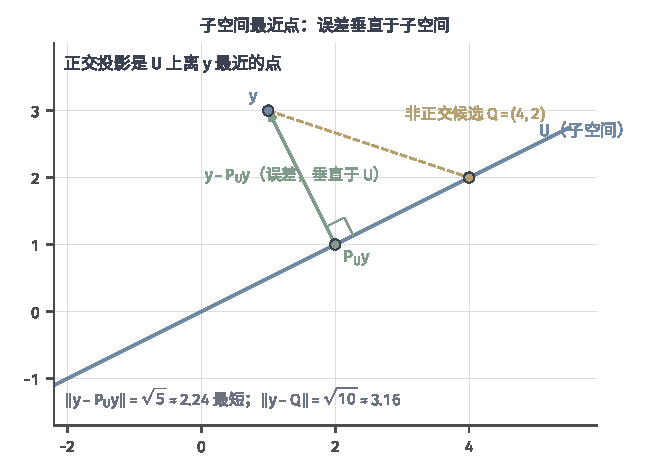
\includegraphics[width=112mm]{figures/01-mathematical-preliminaries-upper/02-linear-spaces/matplotlib/ls-orthogonal-projection-nearest/ls-orthogonal-projection-nearest.pdf}
  \caption{直线子空间$U$（过原点、方向$(2,1)$）上离$\bm y=(1,3)^\top$最近的点是正交投影
  $\bm p=(2,1)^\top$，误差$\bm y-\bm p=(-1,2)^\top$与$U$垂直（直角小方块）；
  同一线上的另一候选$\bm q=(4,2)^\top$到$\bm y$的距离$\sqrt{10}$明显大于最短距离$\sqrt5$。
  这是解析式教学构造。}
  \label{fig:ls-orthogonal-projection-nearest}
\end{figure}

\subsection{求解方法}

\subsubsection{正交化与QR分解}
\label{sec:ls-orthogonalization-qr}

一组向量$\bm q_1,\ldots,\bm q_r$若满足$\langle\bm q_i,\bm q_j\rangle=\delta_{i,j}$，即两两正交且长度为$1$，就称为标准正交组；它的Gram矩阵是单位阵，因而线性无关。张成$U$的标准正交组称为$U$的\term{标准正交基}（orthonormal basis）。
若$U$已有标准正交基$\bm q_1,\ldots,\bm q_r$，系数直接由内积读取：
$\bm p=\sum_j\bm q_j\langle\bm q_j,\bm y\rangle$，每个系数互不干扰。一般基没有这个
便利：基向量夹成斜坐标系，一个方向上的读数混入其他方向，逐个内积不能直接得到
独立系数。所以先把$\bm B$的列整理成正交列与上三角系数的乘积（QR分解），
再读取分量；这一步是把斜坐标换成直角坐标，而不改变点集$U$。

\paragraph{逐方向扣除与Gram--Schmidt}

\term{Gram--Schmidt正交化}按列进行。对$\bm b_j$，先减去它在已有正交方向上的分量：
\begin{equation}
 \bm v_j=\bm b_j-\sum_{i<j}\bm q_i\langle\bm q_i,\bm b_j\rangle,
 \qquad
 \bm q_j=\frac{\bm v_j}{\lVert\bm v_j\rVert_2}.
 \label{eq:ls-classical-gs}
\end{equation}
对$i<j$，$\langle\bm q_i,\bm v_j\rangle
=\langle\bm q_i,\bm b_j\rangle-\langle\bm q_i,\bm b_j\rangle=0$，
故每步$\bm v_j$与先前全部$\bm q_i$正交，归一化后得到新的标准正交方向；
归纳可知$\bm q_1,\ldots,\bm q_j$标准正交且与$\bm b_1,\ldots,\bm b_j$张成同一空间。
例如$\bm b_1=(1,0)^\top$直接给出$\bm q_1=(1,0)^\top$；
$\bm b_2=(1,1)^\top$扣除$\langle\bm q_1,\bm b_2\rangle\bm q_1=(1,0)^\top$后
得$\bm v_2=(0,1)^\top$，归一化即$\bm q_2=(0,1)^\top$。

\paragraph{正交列和上三角系数的形成}

把$\bm b_j=\sum_{i\leq j}r_{i,j}\bm q_i$中的系数$r_{i,j}=\langle\bm q_i,\bm b_j\rangle$
排成上三角矩阵$\bm R$，即得经济型\term{QR分解}
\begin{equation}
 \bm B=\bm Q\bm R,\qquad
 \bm Q^\top\bm Q=\bm I_r,\quad\bm R\text{ 上三角且对角元为正}.
 \label{eq:ls-qr-factorization}
\end{equation}
$\bm Q\in\mathbb R^{m\times r}$的列张成$U$，$\bm R$记录每列相对正交方向的组合系数。
图~\ref{fig:vol1-add-linear-qr-columns}给出最小的二维情形：保留第一条单位方向，
再从第二列减去它在第一方向上的分量，列空间不变，减去的部分记进$\bm R$。
\begin{figure}[!htb]
  \centering
  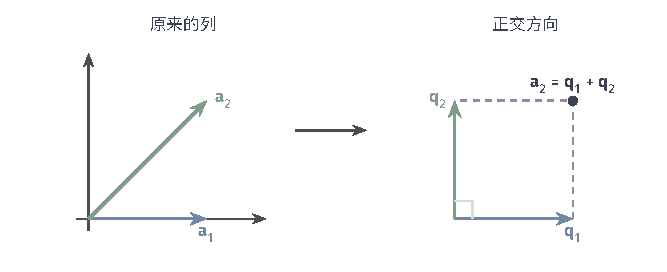
\includegraphics[width=112mm]{figures/01-mathematical-preliminaries-upper/02-linear-spaces/tikz/comprehension-additions/linear-qr-columns.pdf}
  \caption{QR把列的方向和组合系数分开。取$\bm a_1=(1,0)^\top$、$\bm a_2=(1,1)^\top$，
  正交化得到$\bm q_1=(1,0)^\top$、$\bm q_2=(0,1)^\top$，并有$\bm a_1=\bm q_1$、
  $\bm a_2=\bm q_1+\bm q_2$，故$\bm R=\left[\begin{smallmatrix}1&1\\0&1\end{smallmatrix}\right]$。
  虚线补出第二列的分量。}
  \label{fig:vol1-add-linear-qr-columns}
\end{figure}

若$\bm v_j=\bm0$，说明$\bm b_j$已由此前方向张成，输入列线性相关。
此时跳过该列、不执行归一化，或在$\bm R$中保留零系数位置；关键是不能用零向量作除数，
也不能把零长度当成正交失败而中断。归纳看$\bm v_j=\bm0$等价于
$\bm b_j\in\operatorname{span}\{\bm q_1,\ldots,\bm q_{j-1}\}$，空间没有扩大，
故跳过不影响后续列的投影。秩亏时仍得到$\bm B=\bm Q\bm R$，但$\bm R$奇异，
不能当作可逆三角矩阵回代；最近点$\bm p$作为$U$中的点仍唯一，但基系数不唯一，
需另选代表。例如$\bm b_1=(1,0)^\top$、$\bm b_2=(2,0)^\top$，
扣除后$\bm v_2=\bm b_2-2\bm q_1=\bm0$，跳过$\bm b_2$后$U$仍为$x$轴；
若强行归一化零向量会出现$0/0$。

\term{修正Gram--Schmidt}（modified Gram--Schmidt）
在每列扣除时，从当前残差出发依次向所有已有$\bm q_i$投影并立即更新残差，而不是
一次性减去全部旧分量：先$\bm v\leftarrow\bm b_j$，对$i=1,\ldots,j-1$逐次
$r_i=\bm q_i^\top\bm v$、$\bm v\leftarrow\bm v-r_i\bm q_i$，最后归一化。
精确算术中它与经典形式给出同一组正交方向；有限精度下，逐次更新残差使后续投影
基于已扣除的最新残差，正交性损失通常小于一次性扣除，差异由后续数值章节分析。

\paragraph{Householder反射的消元构造}

稠密计算常用\term{Householder反射}一次消去一列主对角线下的全部元素。
对非零实向量$\bm a$，取$s=1$当$a_1\geq0$否则$s=-1$，令
\begin{equation}
 \bm v=\bm a+s\lVert\bm a\rVert_2\bm e_1,\qquad
 \bm H=\bm I-2\frac{\bm v\bm v^\top}{\bm v^\top\bm v}.
 \label{eq:ls-householder}
\end{equation}
直接相乘可验$\bm H^\top\bm H=\bm I$（$\bm v$方向上反射两次回到原向量，
正交方向不变），且$\bm H\bm a=-s\lVert\bm a\rVert_2\bm e_1$：$\bm v$与
$\bm a+s\lVert\bm a\rVert_2\bm e_1$平行，反射把$\bm a$送到其关于该方向的镜像。
符号选择$s=\operatorname{sgn}(a_1)$避免在$\bm v$首元素中相减两个接近的数
（否则有效数字损失）。反射只作用于剩余子块，只需保存反射向量$\bm v$即可依次
应用$\bm H$，不必存整个$m\times m$正交矩阵。
例如$\bm a=(3,4)^\top$，$a_1>0$取$s=1$，$\lVert\bm a\rVert=5$，
$\bm v=(8,4)^\top$，$\bm v^\top\bm v=80$，
$\bm H=\bm I-2\bm v\bm v^\top/80$，计算得
$\bm H=\left[\begin{smallmatrix}-3/5&-4/5\\-4/5&3/5\end{smallmatrix}\right]$，
乘$\bm a$得$(-5,0)^\top$，确实把$\bm a$送到水平轴。

\paragraph{Givens旋转与局部消元}

\term{Givens旋转}在坐标$(i,j)$平面内作旋转，只消去一个指定元素：
\begin{equation}
 \bm G(i,j,\theta)=
 \begin{bmatrix}
  &\ddots&&\ddots\\
  &c&&s\\
  &&\ddots\\
  &-s&&c\\
  &&&\ddots
 \end{bmatrix},
 \qquad c^2+s^2=1,
 \label{eq:ls-givens}
\end{equation}
它只混合第$i,j$两个坐标，其余分量不变。选择$c,s$使第$j$坐标被旋到第$i$坐标、
目标位置归零：对$(a_i,a_j)$取$r=\sqrt{a_i^2+a_j^2}$，
$c=a_i/r$、$s=a_j/r$。新的一对分量为
$(c a_i+s a_j,\,-s a_i+c a_j)$，第二式$-s a_i+c a_j=0$，
第一式$c a_i+s a_j=r$。以$(a_i,a_j)=(3,4)$为例，$r=5$，
$c=3/5$、$s=4/5$，第一分量$c a_i+s a_j=9/5+16/5=5$，
第二分量$-s a_i+c a_j=-12/5+12/5=0$，变换后该对变为$(5,0)$，
非零元素只留在第$i$位置。$r=0$时两坐标已为零，
直接跳过、不必构造旋转。它改动范围小，适合稀疏、带状矩阵和逐列增量更新，
也是后文小型最小二乘问题逐步QR更新的工具；与Householder一次消去整列相比，
Givens每次只消一个元素，运算量更大但只触碰局部非零结构，稀疏优势明显。
图~\ref{fig:ls-givens-householder-elimination}把两种初等正交变换并置：
左图Givens旋转沿圆弧把$(a,b)=(2,1)^\top$旋到$(r,0)^\top$，右图Householder反射
沿角平分线把它映到同一位置，二者都保持长度而只改方向。

\begin{figure*}[htbp]
  \centering
  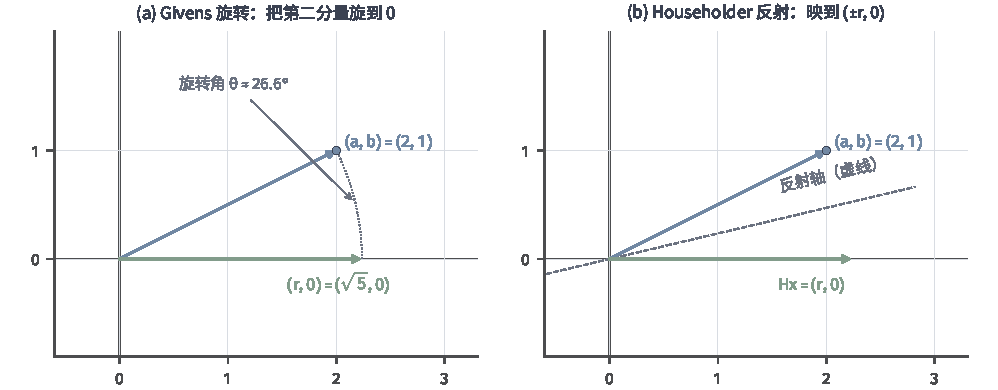
\includegraphics[width=168.998mm]{figures/01-mathematical-preliminaries-upper/02-linear-spaces/matplotlib/ls-givens-householder-elimination/ls-givens-householder-elimination.pdf}
  \caption{两种初等正交消元。左：Givens旋转把$(a,b)=(2,1)^\top$沿圆弧旋到
  $(r,0)^\top$，$r=\sqrt5$，旋转角$\theta=\arctan(1/2)$；右：Householder反射沿角平分线
  把同一向量映到$(r,0)^\top$。两者都是正交变换，保持长度，区别在旋转（行列式$+1$）与
  反射（对称正交）。解析式教学构造。}
  \label{fig:ls-givens-householder-elimination}
\end{figure*}

稠密$m\times d$矩阵的QR约需$2md^2-2d^3/3$次基本浮点运算，
正交列可由反射向量隐式保存，多个右端可以复用全部反射与$\bm R$，
新增一列只需对已有$\bm Q$追加一次投影与正交化，不必整体重做。
稀疏情形按非零结构只触碰局部元素，Givens适合这种逐元素增量更新。
秩亏时QR表示仍然成立，但回代与秩判断需要列置换（选最大模列提前作主元）等补充手段，
判定小$\lvert r_{j,j}\rvert$是数值精度问题而非精确代数结论，阈值与扰动由后续章节
说明。经济型QR只保留$r$列$\bm Q$，节省$m-r$列存储。

\subsubsection{最近点计算}

把候选点写成$\bm p=\bm B\bm c$。存在性一节的反向判据把
“最小距离”换成可直接检验的正交条件：最近点的残差$\bm r=\bm y-\bm B\bm c$必须与
每个基向量$\bm b_i$正交。这个条件不要求预先知道最小值，也不要求对$\bm c$逐点
比较距离，只要求列出$\dim U$个正交方程，把连续最小化变成线性系统求解；它是
可直接核验的一阶条件，满足时由勾股恒等式自动保证全局最小。几何上，残差垂直落
到$U$上，垂足即最近点。

\paragraph{正交残差条件与Gram系统}

标准内积下条件为$\bm B^\top(\bm y-\bm B\bm c)=\bm0$，即
\begin{equation}
 \bm G\bm c=\bm B^\top\bm y,\qquad
 g_{i,j}=\langle\bm b_i,\bm b_j\rangle.
 \label{eq:ls-gram-system}
\end{equation}
逐行写就是$\sum_j\langle\bm b_i,\bm b_j\rangle c_j=\langle\bm b_i,\bm y\rangle$，
即残差与每个基向量正交的$\dim U$个方程。加权内积下改为
$\bm B^\top\bm M(\bm y-\bm B\bm c)=\bm0$，Gram矩阵换成$\bm B^\top\bm M\bm B$。
\ref{sec:ls-orthogonality}已说明：基向量线性无关时，对任意非零$\bm c$有
$\bm c^\top\bm G\bm c=\lVert\bm B\bm c\rVert_2^2>0$，故$\bm G$正定、系统可逆。
边界：若基相关，$\bm G$奇异，方程仍相容但系数不唯一，最近点作为点仍唯一。

$\bm G$正定时方程~\eqref{eq:ls-gram-system}有唯一解$\bm c$，
对应唯一最近点$\bm p=\bm B\bm c$；权重$\bm M$正定时加权Gram矩阵
$\bm B^\top\bm M\bm B$同样正定（对非零$\bm c$有
$\bm c^\top\bm B^\top\bm M\bm B\bm c=\lVert\bm B\bm c\rVert_{\bm M}^2>0$），
同一结论保持。基相关时$\bm G$奇异、系数不唯一（同一$\bm p$
有多种组合），但最近点$\bm p$作为$U$中的点仍唯一，只需要再按准则选系数代表；
例如$\bm b_2=2\bm b_1$时，$\bm p=\bm b_1$可写成$\bm c=(1,0)$或$(0,1/2)$，
点相同而系数不同。

由$\bm B=\bm Q\bm R$，$\bm R$可逆时$\bm p=\bm Q\bm Q^\top\bm y$：
先算$\bm Q^\top\bm y$，再解三角系统$\bm R\bm c=\bm Q^\top\bm y$恢复系数，
最后$\bm p=\bm B\bm c$。由于$\bm Q^\top\bm Q=\bm I$，
$\bm Q^\top\bm y$的分量就是各正交方向上的坐标，无需先解Gram系统。
这条路线不显式形成Gram矩阵；形成正规乘积造成的尺度损失由后续章节用条件数解释。

核验分三步：$\bm p=\bm B\bm c\in U$；残差$\bm r=\bm y-\bm p$与$\bm B$各列正交；
报告最小距离$\lVert\bm r\rVert_2$。加权内积改变最近点，例~\ref{ex:linear-algebra-weighted-projection}
在同一直线上比较两种度量。
\begin{example}[同一子空间的两种最近点]
\label{ex:linear-algebra-weighted-projection}
在$\mathbb R^2$中取目标$\bm y=(2,1)^\top$、$U=\operatorname{span}\{(1,1)^\top\}$，
最近点写成$a(1,1)^\top$。欧氏投影最小化$(2-a)^2+(1-a)^2$，
导数给出$2a=3$，故$\bm p=(1.5,1.5)^\top$。
改用$\bm M=\operatorname{diag}(1,4)$，目标函数为$(2-a)^2+4(1-a)^2$，
导数给出$10a=12$，即$5a=6$，得到$\bm p_{\bm M}=(1.2,1.2)^\top$。
第二坐标误差代价更大，最近点便向$b_2=1$靠近；
残差$(0.8,-0.2)^\top$与$(1,1)^\top$的普通内积为$0.6\neq0$，
加权内积$0.8\cdot1+4(-0.2)\cdot1=0$，正交性必须用所选内积判断。
\end{example}
\begin{figure*}[htbp]
  \centering
  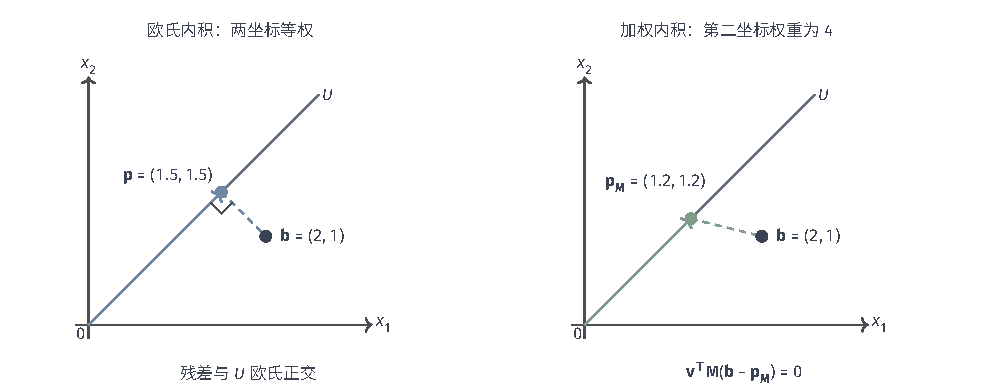
\includegraphics[width=168.998mm]{figures/01-mathematical-preliminaries-upper/02-linear-spaces/tikz/linear-algebra-weighted-projection/figure.pdf}
  \caption{同一目标在同一直线上的欧氏投影与加权投影。实箭头是投影向量，虚线是残差；
  右图画在普通坐标中，残差不必形成欧氏直角。正交性必须用所选内积判断。}
  \label{fig:linear-algebra-weighted-projection}
\end{figure*}

\subsection{投影的性质}

\paragraph{正交投影、斜投影与幂等}

标准内积下，以$\bm Q$为标准正交基的正交投影为
\begin{equation}
 \bm P_U=\bm Q\bm Q^\top,\qquad
 \bm P_U^\top=\bm P_U,\qquad \bm P_U^2=\bm P_U.
 \label{eq:linear-algebra-orthogonal-projector}
\end{equation}
它同时满足三条可逐条核验的性质：
\begin{enumerate}
 \item \term{幂等}（idempotent）：$\bm P_U^2=\bm Q\bm Q^\top\bm Q\bm Q^\top=\bm Q\bm Q^\top$，
 作用两次等于作用一次。
 \item 自伴（标准内积下$\bm P_U^\top=\bm P_U$）：保证残差与像正交，即欧氏最近点。
 \item 像为$U$：$\operatorname{range}\bm P_U=\operatorname{range}\bm Q=U$。
\end{enumerate}
但一般幂等映射只是沿某个方向把空间投到像上，
残差不必与像正交，也未必是最近点，这种映射称为\term{斜投影}（oblique projection）；
只有自伴的幂等映射才是正交投影。
例如$\bm P=\left[\begin{smallmatrix}1&-1\\0&0\end{smallmatrix}\right]$满足
$\bm P^2=\bm P$，把$(x,y)^\top$投到$x$轴上的$(x-y,0)^\top$，但
$\bm P^\top\neq\bm P$，残差$(y,y)^\top$不与$x$轴正交（普通内积$y\cdot0+y\cdot1=y\neq0$），
因而不是欧氏最近点。判别顺序：先验幂等（是否投影），再验对称（是否正交），
不能见幂等就当作最近点映射。

两个正交投影的复合一般不可交换：$\bm P_U\bm P_V\neq\bm P_V\bm P_U$，
乘积也未必仍是投影（两次投影的像一般既不是$U$也不是$V$）。两者可交换时，乘积
幂等且自伴，其像为$U\cap V$。反复投影怎样收敛到交空间属于序列极限问题，
留给后续收敛章节分析，这里不声称一次复合给出极限。

\section{线性方程：精确求解}
\label{sec:ls-exact-linear-equations}
\label{sec:linear-algebra-exact-systems}

\subsection{方程与条件}

给定$\bm A\in\mathbb R^{m\times d}$与目标$\bm b\in\mathbb R^m$，精确方程为
\begin{equation}
 \bm A\bm x=\bm b,\qquad \bm x\in\mathbb R^d.
 \label{eq:linear-algebra-linear-system}
\end{equation}
多个右端写成$\bm A\bm X=\bm B$，$\bm X\in\mathbb R^{d\times s}$、$\bm B\in\mathbb R^{m\times s}$；
它逐列等价于$s$个同系数矩阵的单右端方程$\bm A\bm x_j=\bm b_j$。
同一个$\bm A$的分解或迭代设置可按列复用，但每一列的相容性与残差要分别核验，
不能用一列的残差代替另一列。

按形状分：$m=d$为方阵，$m>d$为超定（方程多于未知量），$m<d$为欠定。
形状只限制秩的上限，不能单独判断有没有解：例如$\bm A=\left[\begin{smallmatrix}1\\1\end{smallmatrix}\right]$
是超定系统，但$\bm b=(1,1)^\top$在列空间内，因而相容且唯一；
而两行相同的方阵$\bm A=\left[\begin{smallmatrix}1&1\\1&1\end{smallmatrix}\right]$配
$\bm b=(1,2)^\top$就不相容。是否存在解由右端与值域的关系决定，
是否唯一由零空间决定，下面先判这两件事。

本节要求等式严格成立；浮点计算中“精确”表现为残差小到
给定容限，容限取值、舍入积累与条件数由后续章节处理。这里先在代数层面区分无解、
唯一解与多解，不能由某个算法算不出解就推断问题无解——算法失败可能只是数值或
实现问题，与代数相容性是两回事。

\subsection{存在性、唯一性与选解}

\subsubsection{相容性}
\label{sec:ls-compatibility}

$\bm A\bm x$是$\bm A$各列以$\bm x$为系数的线性组合，因此
$\bm A\bm x=\bm b$有解当且仅当$\bm b\in\operatorname{range}(\bm A)
=\operatorname{span}\{\bm a_1,\ldots,\bm a_d\}$。这一条件称为\term{相容}
（consistent）；不相容时任何输入都不能精确产生$\bm b$。判据直接来自列空间定义：
可达输出恰好是列的全部线性组合。例如$\bm A=\left[\begin{smallmatrix}1&1\\0&1\end{smallmatrix}\right]$，
两列$(1,0)^\top,(1,1)^\top$线性无关，列空间是全$\mathbb R^2$，任意右端都可达；
若把第二列换成$(1,1)^\top$使两列相同，列空间只是一条直线，垂直于它的右端就
不可达。形状（方程数多少）不决定可达性，列张成的空间才决定。

标准内积下有四个基本子空间：值域$\operatorname{range}(\bm A)$
与零空间$\operatorname{null}(\bm A)=\{\bm x:\bm A\bm x=\bm0\}$，
行空间$\operatorname{range}(\bm A^\top)$与左零空间
$\operatorname{null}(\bm A^\top)=\{\bm y:\bm A^\top\bm y=\bm0\}$。
由\ref{sec:ls-adjoints}建立的伴随恒等式
$\langle\bm y,\bm A\bm x\rangle=\langle\bm A^\top\bm y,\bm x\rangle$
是下面正交互补关系的依据：它把输出空间的配对转成输入空间的配对，使两个正交
关系不必另行假设。四个子空间分属输入、输出两个空间，不要混在同一侧。

若$\bm y\in\operatorname{null}(\bm A^\top)$，则对任意$\bm x$有
$\bm y^\top(\bm A\bm x)=(\bm A^\top\bm y)^\top\bm x=0$，故
$\operatorname{null}(\bm A^\top)\subseteq\operatorname{range}(\bm A)^\perp$；
维数互补给出反向包含，于是
\begin{equation}
 \operatorname{range}(\bm A)^\perp=\operatorname{null}(\bm A^\top).
 \label{eq:ls-range-leftnull-orthogonal}
\end{equation}

同理，$\operatorname{range}(\bm A^\top)^\perp
=\operatorname{null}(\bm A)$：若$\bm x\in\operatorname{null}(\bm A)$，则对任意
$\bm A^\top\bm y$有$(\bm A^\top\bm y)^\top\bm x=\bm y^\top\bm A\bm x=0$，
反向包含由维数互补得到。输入空间因此正交直和分解为
$\operatorname{null}(\bm A)\oplus\operatorname{range}(\bm A^\top)$，
输出空间分解为$\operatorname{range}(\bm A)\oplus\operatorname{null}(\bm A^\top)$。
前者记录被映射消去的输入方向，后者记录达不到的输出方向。

$\bm A\bm x=\bm b$相容的几何判据是$\bm b\in\operatorname{range}(\bm A)$，
即$\bm b$落在列空间内。等价地，由式~\eqref{eq:ls-range-leftnull-orthogonal}，
$\bm b$与左零空间正交：$\bm y^\top\bm b=0$对一切$\bm y\in\operatorname{null}(\bm A^\top)$
成立。前面的最近点结果将用于：不相容时求离$\bm b$最近的可达输出，
这是后续最小二乘任务的入口；本节只在相容前提下求精确解，不做残差最小化，
也不把“最近点”冒充为“解”。判据对任意形状的$\bm A$都适用，与$m,d$谁大无关。

\paragraph{增广矩阵的秩判据}

把$\bm b$并入系数矩阵得到增广矩阵$[\bm A\;\bm b]$。
$\bm b$是列的组合，当且仅当并入它不增加列空间维数，即
\begin{equation}
 \operatorname{rank}[\bm A\;\bm b]=\operatorname{rank}(\bm A).
 \label{eq:ls-augmented-rank}
\end{equation}
这是消元可直接检验的代数判据；不等号出现即无解。理由：若$\bm b$已在列空间内，
并入不扩大张成空间，秩不变；否则秩增加一。例如
$\bm A=\left[\begin{smallmatrix}1&1\\1&1\end{smallmatrix}\right]$的秩为$1$，
$\bm b=(1,2)^\top$使$[\bm A\;\bm b]$秩为$2$，判据直接给出无解；
而$\bm b=(1,1)^\top$并入后秩仍为$1$，相容。

不相容可由左零空间直接证明：若存在
$\bm y\in\operatorname{null}(\bm A^\top)$使$\bm y^\top\bm b\neq0$，
则所有可达输出$\bm A\bm x$在$\bm y$方向读数为
$\bm y^\top\bm A\bm x=(\bm A^\top\bm y)^\top\bm x=0$，而$\bm b$非零，
故$\bm b$不可达。上例中$\bm y=(1,-1)^\top$满足
$\bm A^\top\bm y=0$，而$\bm y^\top\bm b=1-2=-1\neq0$，这就是不可达证书。
反之，$\bm y^\top\bm b=0$对全部$\bm y\in\operatorname{null}(\bm A^\top)$
成立时，由式~\eqref{eq:ls-range-leftnull-orthogonal}知$\bm b$与左零空间正交，
即$\bm b\in\operatorname{range}(\bm A)$。证书法与秩判据等价，但给出一个可
直接核验的向量。

$\bm A\bm X=\bm B$相容当且仅当每一列
$\bm b_j\in\operatorname{range}(\bm A)$，等价于
$\operatorname{rank}[\bm A\;\bm B]=\operatorname{rank}(\bm A)$，
也等价于所有$\bm y\in\operatorname{null}(\bm A^\top)$满足$\bm y^\top\bm B=\bm0$。
各列独立判断，不能用一列相容代替另一列；逐列残差分别核验。

\subsubsection{唯一性与自由度}
\label{sec:ls-uniqueness-freedom}

设$\bm x_1,\bm x_2$都是解，则
$\bm A(\bm x_1-\bm x_2)=\bm b-\bm b=\bm0$，两解之差属于零空间
$\operatorname{null}(\bm A)$；反之，若$\bm x_0$是解且
$\bm n\in\operatorname{null}(\bm A)$，则$\bm A(\bm x_0+\bm n)=\bm b+\bm0=\bm b$，
故$\bm x_0+\bm n$也是解。这一双向关系说明：解集合恰好是“一个特解平移零空间”，
没有其他点混入。

\paragraph{特解加零空间的全部解}

相容时任取一个特解$\bm x_0$，全部解恰为
\begin{equation}
 \bm x=\bm x_0+\operatorname{null}(\bm A).
 \label{eq:ls-affine-solution-set}
\end{equation}
这是一个平移后的线性子空间，即\term{仿射空间}（affine space）：基点$\bm x_0$
不唯一，更换基点只平移集合，方向空间$\operatorname{null}(\bm A)$由全部点差唯一确定。
商空间把这种不可区分性表达为精确对应：
$\mathbb R^d/\operatorname{null}(\bm A)\to\operatorname{range}(\bm A)$，
$\bm x+\operatorname{null}(\bm A)\mapsto\bm A\bm x$良定义、线性、单射且满射，
却尚未在每个类中选代表。例如$x_1+x_2=2$有特解$(1,1)^\top$，零空间由
$(1,-1)^\top$张成，全部解为$(1,1)^\top+t(1,-1)^\top$，$t$任意；
$(1,0)^\top$与$(0,1)^\top$在$\bm A=(1,1)$下同属一类、只记录系数和。
\label{sec:linear-algebra-affine-relations}
图~\ref{fig:vol1-add-linear-nullspace-fibers}以$\bm A=(1,1)$展示：每条平行线
$x_1+x_2=c$对应同一个输出数，整条线归为一个原像类。
\begin{figure}[!htb]
  \centering
  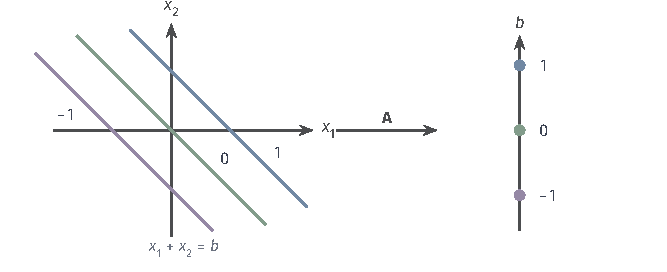
\includegraphics[width=112mm]{figures/01-mathematical-preliminaries-upper/02-linear-spaces/tikz/comprehension-additions/linear-nullspace-fibers.pdf}
  \caption{同一输出对应的整组输入。对$\bm A=(1,1)$，蓝、绿、紫直线分别满足
  $x_1+x_2=1,0,-1$；右侧同色点是各直线的输出。绿色直线是$\ker\bm A$，
  其余直线是它的平移。把一整条直线归为一类后，才得到与可达输出的一一对应。}
  \label{fig:vol1-add-linear-nullspace-fibers}
\end{figure}

由秩零度定理~\ref{thm:ls-rank-nullity}，
$\dim\operatorname{null}(\bm A)=d-\operatorname{rank}(\bm A)$，
这就是自由参数的个数。相容时任一特解$\bm x_0$加上零空间的全部点构成解集，
解集是$d-r$维仿射空间，$r=\operatorname{rank}(\bm A)$；
每增加一个自由参数，就多一个沿零空间移动而不改变输出的方向，自由参数个数
与列数减秩一致。例如$\bm A=[1\ 1]$，$d=2,r=1$，自由参数$1$个，
解$\bm x=(1,1)^\top+t(1,-1)^\top$中$t$即自由参数；$d-r=0$时零空间只含零向量，
自由参数为零，解唯一。

\paragraph{满列秩、满行秩与唯一性}

解唯一当且仅当$\operatorname{null}(\bm A)=\{\bm0\}$，
即满列秩$r=d$（$d$个列向量线性无关）：两解之差落在零空间，零空间为零向量迫使
两解相同。满行秩$r=m$只保证每个右端都可达（相容），
不保证唯一；满列秩保证唯一但不保证任意右端可达。两种满秩对应不同保证，
不能互换：满行秩可能欠定多解，满列秩可能超定不相容。例如$\bm A=(1,1)$满行秩
（$m=1$）但欠定，任意$\bm b$相容而解不唯一；$\bm A=(1,1)^\top$满列秩（$d=1$），
解唯一却只对$\bm b\in\operatorname{span}\{(1,1)^\top\}$相容。

超定$m>d$且满列秩时，相容则唯一解，不相容则无精确解（此时进入残差最小化任务）；
欠定$m<d$且满行秩时任意右端都相容，但至少有$d-m$个自由参数，解不唯一。
仅凭方程数与未知数个数不能下结论，必须回到实际秩与右端位置：超定也可能相容唯一，
方阵也可能无解。例如方阵$\bm A=\left[\begin{smallmatrix}1&1\\1&1\end{smallmatrix}\right]$
秩$1<d=2$，既多解又对$\bm b\notin\operatorname{span}\{(1,1)^\top\}$无解，
形状为方阵却不具备可逆性。

$\bm A=\bm0$时：$\bm b=\bm0$则任意$\bm x$都是解
（零空间为全空间$\mathbb R^d$，列空间为$\{0\}$），$\bm b\neq\bm0$则无解
（零右端落在列空间$\{0\}$内，非零右端不在）。反过来$\bm b=\bm0$而$\bm A\neq0$
时齐次方程$\bm A\bm x=\bm0$恒相容，至少有零解，秩亏时另有非零解。
这种边界不能套用含零分母的求逆公式（$\bm A^{-1}$不存在），直接按上述秩与值域
判据判断，避免对零矩阵作除法。

\subsubsection{多解中的选择}
\label{sec:ls-select-among-solutions}

相容而秩亏时，全部解是$\bm x_0+\operatorname{null}(\bm A)$，
等式本身不再挑选代表，需要额外准则。常用的是在解集中取欧氏范数最小者；
更换输入内积，代表点一般随之改变，准则必须先声明，不能默认“解”唯一。
这一准则与6.1的最近点几何一致：在平移仿射集合上找离原点最近的点，
垂足落在零空间的正交补上。

把任意解按输入空间的正交直和分解为
$\bm x=\bm x_\perp+\bm x_N$，其中$\bm x_N\in\operatorname{null}(\bm A)$，
$\bm x_\perp\in\operatorname{null}(\bm A)^\perp=\operatorname{range}(\bm A^\top)$。
$\bm A\bm x_N=\bm0$，输出只由$\bm x_\perp$决定，核分量对输出毫无贡献；
两个分量正交，故可分开处理。

\paragraph{最小范数精确解的唯一性}

两项正交，故
$\lVert\bm x\rVert_2^2=\lVert\bm x_\perp\rVert_2^2+\lVert\bm x_N\rVert_2^2$。
保持$\bm x_\perp$不变而去掉$\bm x_N$，输出不变（$\bm A\bm x_N=0$）且范数
严格减小；唯一最小范数代表就是$\bm x_N=0$的那个解，它落在
$\operatorname{null}(\bm A)^\perp$中。上例$x_1+x_2=2$的解
$(1+t,1-t)^\top$中，范数平方为$(1+t)^2+(1-t)^2=2+2t^2$，令核分量$t=0$
得$(1,1)^\top$，其范数$\sqrt2$小于$t\neq0$时的$\sqrt{2+2t^2}$。
映射$\bm A|_{\operatorname{null}(\bm A)^\perp}:
\operatorname{null}(\bm A)^\perp\to\operatorname{range}(\bm A)$是双射：
单射来自交为零，满射来自上述分解，故最小范数代表存在且唯一。

满列秩时$\bm A^\top\bm A$正定，存在左逆
$\bm L=(\bm A^\top\bm A)^{-1}\bm A^\top$使$\bm L\bm A=\bm I$，
它能恢复全部输入，但只对值域中的输出反演；满行秩时存在右逆
$\bm R=\bm A^\top(\bm A\bm A^\top)^{-1}$使$\bm A\bm R=\bm I$，
它为每个输出挑一个输入，却不能恢复被零空间消去的信息。单侧逆一般不唯一：
例如$\bm A=(1,0)^\top$，任意$\bm L=(1,t)$都满足$\bm L\bm A=1$，
$t$任意而不破坏左逆。它们是代数公式，实际通过三角求解应用，不显式形成逆矩阵；
左逆对应唯一解（满列秩），右逆对应一种选解（满行秩）。

最小范数代表依赖指定的输入内积；一般权重或正则化会同时改变目标与代表，
完整的伪逆构造、任意秩处理与加权选解放在后续残差最小一节。本节只确认：多解时等式不唯一，
必须先声明准则再谈“解”；在未声明准则前，报告“一个解”而非“那个解”。
满行秩右逆给出的代表只是众多选解之一，未必是最小范数代表，二者不可混称。

\subsection{直接法}
\label{sec:ls-direct-methods}
\label{sec:linear-algebra-direct-exact}
\label{sec:matrix-analysis-stable-solvers}

直接法在有限步内把方程化为可逐个求解的三角或块系统。它需要显式读取并存储因子，
适用于矩阵可整体获得、规模可控或多右端复用同一因子的情形。

\subsubsection{消元与LU分解}

高斯消元用一行的倍数消去另一行的某个系数，
行变换（把某行加到另一行、交换两行、某行乘非零常数）不改变解集。例如
$\left[\begin{smallmatrix}2&1\\4&3\end{smallmatrix}\right]\bm x=(1,3)^\top$，
第二行减去第一行的两倍得$(0,1)$对应$x_2=1$，再代回$2x_1+1=1$得$x_1=0$。
多步消元记录下来就是三角因子，不必每次从头回代。

第$k$步在尚未处理的第$k$列中选择绝对值最大的可用元素移到主元位置，
再消去它下方的元素；记录的行交换累计为置换矩阵$\bm P$。例如主元位置为零而其下方
同列有非零元时，交换两行即可继续；部分主元避免把本可交换避开的零元素拿来作除数，
也抑制乘子$l_{i,k}=a_{i,k}/a_{k,k}$过大带来的放大。但交换不会把奇异矩阵变成
可逆矩阵：秩由列张成决定，行置换只重排方程，不改变秩与相容性。

\paragraph{消元乘子与LU因子}

消去乘子$l_{i,k}=a^{(k)}_{i,k}/a^{(k)}_{k,k}$进入单位下三角
因子$\bm L$，剩余系数构成上三角因子$\bm U$，得到带部分主元的分解
\begin{equation}
 \bm P\bm A=\bm L\bm U,
 \label{eq:matrix-analysis-palu}
\end{equation}
其中$\bm L$单位下三角（对角为1）、$\bm U$上三角。乘子就是第$k$步消去第$i$行
第$k$列所用的倍数，被原样留在$\bm L$中，使$\bm L\bm U$乘回可复原置换后的
系数矩阵；前面列的乘子随行交换同步更新。验证方式：把$\bm L\bm U$逐项乘回，
与$\bm P\bm A$比较，不必另行求解。

消元得到的阶梯形直接显示秩：每选到一个非零主元秩加一；精确算术中某列无可用主元，
说明矩阵秩亏，此时应转入秩判断并按6.2.1相容性判据核验增广矩阵秩，而不是继续
除以零。对相容的秩亏系统，自由变量取零即得一个特解，其余解沿零空间展开；
对不相容系统，阶梯形会出现$0=\text{非零}$的矛盾行，直接判定无解。
某个小主元不能独自证明精确奇异，浮点阈值决定的数值秩留待后续章节说明；
代数上的奇异（主元恰为零）与数值上的接近奇异（主元很小但非零）是两件事。

分解后依次解$\bm L\bm z=\bm P\bm b$（前代，从前向后）与
$\bm U\bm x=\bm z$（回代，从后向前）：
\begin{equation}
 z_i=(\bm P\bm b)_i-\sum_{j<i}l_{i,j}z_j,\qquad
 x_i=\frac{z_i-\sum_{j>i}u_{i,j}x_j}{u_{i,i}}.
\end{equation}
回到开头的例子，消元后$\bm U=\left[\begin{smallmatrix}2&1\\0&1\end{smallmatrix}\right]$、
$\bm L=\left[\begin{smallmatrix}1&0\\2&1\end{smallmatrix}\right]$，
先由$\bm L\bm z=(1,3)^\top$得$z_1=1$、$z_2=1$，再回代$x_2=1$、
$2x_1+1=1$得$x_1=0$。解出后代回原方程核验$\bm A\bm x=\bm b$。

因子$\bm L,\bm U$（或置换$\bm P$）只建立一次，每个新右端$\bm b_j$各自完成两次
三角求解$\bm L\bm z_j=\bm P\bm b_j$、$\bm U\bm x_j=\bm z_j$，不必为每列重做
$O(d^3)$分解；当同一$\bm A$搭配多列$\bm B$时，分摊成本主要落在$O(d^2)$的逐列
三角求解上。矩阵改变后不能无条件复用旧因子：结构或元素变化使$\bm L\bm U$不再等于
新的$\bm P\bm A$，须重新分解；仅有右端变化才允许复用。

稠密$d\times d$矩阵的LU分解约需$2d^3/3$次基本浮点运算，
每个新右端的两次三角求解为$O(d^2)$，存储$O(d^2)$。稀疏矩阵消元可能产生原来
没有的非零元，称为\term{填充}（fill-in），使原本稀疏的因子退化为准稠密；
存储收益还取决于行列排序与结构，而不只看原始非零元数。因此稀疏直接法的成本
不能只用原始非零元数估计。

\subsubsection{Cholesky分解}

当$\bm A=\bm A^\top\succ0$（对称正定）时，
定理~\ref{thm:ls-gram-factor}的配方原理已说明正定矩阵可归纳写成$\bm L\bm L^\top$
形式；本节把它落实为可逐列执行的三角求解算法。Cholesky 能省去 LU 的选主元，前提可拆成
三条同时成立：
\begin{enumerate}
 \item 对称性$\bm A=\bm A^\top$：只需存储一个三角因子，配方只作用于上半。
 \item 正定性$\bm x^\top\bm A\bm x>0$（$\bm x\neq\bm0$）：等价于各阶顺序主子式为正，
 配方剩余$a_{j,j}-\sum_{k<j}l_{j,k}^2>0$恒成立。
 \item 由此每步主元严格为正：无需行交换，不会出现零主元或负数开方。
\end{enumerate}
这是它相对LU的简化前提。

把第一个坐标与其余坐标分块配方，消去首变量后剩余的系数矩阵
仍正定，因而每一步的主元严格为正；按维数归纳即可逐列构造因子。具体地，正定二次型
对首变量配成完全平方，平方项系数为正，余下不含首变量的二次型由正定性仍正定，
这也解释了Cholesky每步剩余矩阵为何保持正定结构、根号内为何严格为正。这一归纳
正是定理~\ref{thm:ls-gram-factor}配方原理的逐步执行，不是另立假设。

\paragraph{Cholesky因子的逐列构造}

存在唯一对角元为正的下三角矩阵$\bm L$使
\begin{equation}
 \bm A=\bm L\bm L^\top,
 \label{eq:matrix-analysis-cholesky}
\end{equation}
称为\term{Cholesky分解}（Cholesky decomposition）。逐列计算
\begin{equation}
 l_{j,j}=\sqrt{a_{j,j}-\sum_{k<j}l_{j,k}^2},\qquad
 l_{i,j}=\frac{a_{i,j}-\sum_{k<j}l_{i,k}l_{j,k}}{l_{j,j}}\quad(i>j).
\end{equation}
第一式是第$j$个对角平方（配方剩余），第二式由$\bm L\bm L^\top$的$(i,j)$元
$a_{i,j}=\sum_{k\leq j}l_{i,k}l_{j,k}$反解得到。正定性保证根号内严格为正，
除法合法。例如$\bm A=\left[\begin{smallmatrix}4&2\\2&5\end{smallmatrix}\right]$，
先得$l_{11}=\sqrt4=2$，再$l_{21}=a_{21}/l_{11}=2/2=1$，最后
$l_{22}=\sqrt{5-l_{21}^2}=\sqrt{5-1}=2$，故
$\bm L=\left[\begin{smallmatrix}2&0\\1&2\end{smallmatrix}\right]$，
乘回$\bm L\bm L^\top=\left[\begin{smallmatrix}4&2\\2&5\end{smallmatrix}\right]$
逐项等于原矩阵。

每列由先前列唯一确定：式~\eqref{eq:matrix-analysis-cholesky}的$(i,j)$元给出
$a_{i,j}=\sum_{k\leq j}l_{i,k}l_{j,k}$，右侧$k<j$项已由先前因子确定，故$l_{i,j}$
被唯一反解；对角$l_{j,j}$由配方剩余开方，正对角约定又固定了开方符号（取$+$而非$-$），
因此带正对角的Cholesky分解唯一。若允许对角取负号，$\pm l_{j,j}$都满足乘积，符号未定，
正对角约定排除了这一任意性。对照LU：一般矩阵的LU在主元非零时也唯一，
而Cholesky额外靠正定性保证根号内为正、无需选主元。

求解依次用$\bm L\bm z=\bm b$（前代，$z_i=(b_i-\sum_{j<i}l_{i,j}z_j)/l_{i,i}$）与
$\bm L^\top\bm x=\bm z$（回代，$x_i=(z_i-\sum_{j>i}l_{j,i}x_j)/l_{i,i}$）。
稠密成本约$d^3/3$，只存一个三角因子（利用对称不复存上半），
约为LU的一半；多个右端复用同一因子，每个右端仍需两次三角求解$O(d^2)$。
复用前提仍是$\bm A$不变。

半正定时可能出现零主元（配方剩余为零），不能照搬上述除以$l_{j,j}$与开正根号的
步骤，否则$0/0$或负数开方。盲目加一个“小常数”会改变原方程、把退化系统改成另一
问题；应先区分真实退化（$\bm A$本有零空间、相容前提下进入选解）、约束造成的零空间
与数值误差（接近奇异而非精确奇异，阈值问题留后续章节）。只有任务本身明确引入阻尼
或惩罚时，才改用相应的正则化系统，不能为让算法通过而临时改动系数。

\subsubsection{LDL$^{\top}$分解}
\label{sec:ls-ldlt}

对称但不定（有正也有负方向）的矩阵不能逐项开正平方根：它既没有Cholesky所需的
正主元可开正根号，也没有CG所需的正分母，二者都不能沿用；例如$\operatorname{diag}(1,-1)$可逆却出现负主元，
$\sqrt{-1}$无实意义。对称结构仍然保留，可把符号和耦合
留在对角块中，这正是LDL$^{\top}$分解的用途：不开方、由$\bm D$的负块承接符号。

引入带对称置换的分解$\bm P\bm A\bm P^\top=\bm L\bm D\bm L^\top$，
其中$\bm L$单位下三角，$\bm D$由一阶与二阶对角块组成。
例如$\left[\begin{smallmatrix}0&1\\1&0\end{smallmatrix}\right]$可逆却没有可用的一阶对角主元；
同时交换行列以保留对称性，选择可逆的一阶或二阶块作主元，再消去与剩余变量的耦合。

\paragraph{LDL$^{\top}$因子的形成}

按块递归消去耦合。把当前待消矩阵分块为
$\begin{bmatrix}\bm A_{11}&\bm A_{12}\\\bm A_{21}&\bm A_{22}\end{bmatrix}$，
其中$\bm A_{11}$是选定的可逆一阶或二阶块；单位下三角乘子块取
$\bm L_{21}=\bm A_{21}\bm A_{11}^{-1}$，消去后剩余块为Schur补
$\bm A_{22}-\bm A_{21}\bm A_{11}^{-1}\bm A_{12}$，再对剩余块重复同一过程。
$\bm L$记录这些乘子（单位对角），$\bm D$保留各步选定的对角块（一阶标量或二阶
对称块）。不定矩阵的负主元不是算法失败，只是不能开平方；$\bm D$的负块直接
保留符号。每步乘回$\bm L\bm D\bm L^\top$逐项核对，确认乘积等于置换后的系数矩阵。
与Cholesky相比，LDL$^{\top}$不开根号、把符号集中在$\bm D$，因此可覆盖对称不定
与条件良好的半定情形；$\bm D$为一阶、二阶块正是为了在无正主元时仍取得可逆块。

一阶块$d$直接除以标量$d$：$y=z/d$。二阶块
$\begin{smallmatrix}d_{11}&d_{12}\\d_{12}&d_{22}\end{smallmatrix}$
解$\bm D\bm y=\bm z$，令$\Delta=d_{11}d_{22}-d_{12}^2$（非零由块主元可逆保证），
则
\begin{equation}
 y_1=\frac{d_{22}z_1-d_{12}z_2}{\Delta},\qquad
 y_2=\frac{d_{11}z_2-d_{12}z_1}{\Delta}.
\end{equation}
负对角元照常保留，不要求开平方；二阶块一次解完即可，不必再细分。例如二阶块
$\begin{smallmatrix}0&1\\1&0\end{smallmatrix}$（$d_{11}=0,d_{12}=1,d_{22}=0$）
行列式$\Delta=-1\neq0$，代入得$y_1=z_2$、$y_2=z_1$，直接解出两个未知量，
避免了寻找不存在的一阶零对角主元。

求解依次经过置换（把右端按$\bm P$重排）、下三角系统$\bm L\bm z=\bm P\bm b$
（前代）、小对角块系统$\bm D\bm y=\bm z$（逐块解一阶/二阶）和上三角系统
$\bm L^\top\bm x=\bm y$（回代），最后按置换$\bm P^\top$恢复原坐标；
每一步都是易解的三角或小块系统，回代次序与消元相反，置换把被交换的列/行位置
还原。这一链条与Cholesky两次三角求解平行，只是中间插入块对角求解与逆置换。

区分“具有负方向”（不定、$\bm D$出现负块）和“具有零空间”（奇异、$\bm D$出现
零块）：前者仍可唯一求解，负块只是符号；后者需重新判断相容性与选解，不能把零块
当可逆块作除法。这里只说明结构与求解路径，求解驻点方程不等于最小化对应的二次目标
（不定二次型无下界，驻点不是极小点）。

\subsubsection{QR分解}

前面建立的QR用正交变换把$\bm A$化为上三角。正交变换
保持欧氏长度，对相容方程$\bm A\bm x=\bm b$左乘$\bm Q^\top$后，方程拆成
可解的三角约束（前$d$行$\bm R\bm x=\bm Q^\top\bm b$）与自动满足的零残差行
（下方$\bm Q^\top\bm b$分量为零，这是相容条件$\bm b\in\operatorname{range}(\bm A)$
的投影表达），不需要额外极小化。不相容时下方残差非零，进入最小二乘任务而非本节。

$m\geq d$且满列秩时，经济型$\bm A=\bm Q\bm R$给出
$\bm R$可逆上三角；相容时解$\bm R\bm x=\bm Q^\top\bm b$，下方行的残差自动为零。
例如$\bm A=\left[\begin{smallmatrix}1&1\\1&0\\0&1\end{smallmatrix}\right]$，
两列线性无关；取相容右端$\bm b=(2,1,1)^\top=\bm A(1,1)^\top$。QR把$\bm A$
化为上三角，前两行$\bm R$可逆、第三行为零；左乘$\bm Q^\top$后第三行给出相容性核验
（此处$\bm Q^\top\bm b$第三分量为零），前两行的上三角系统回代得
$\bm x=(1,1)^\top$，代回$\bm A\bm x$得$(2,1,1)^\top=\bm b$。
若右端使第三分量非零，则方程不相容，转入后文最小二乘而非此处三角求解。

$m\leq d$且满行秩时对$\bm A^\top$作QR（即LQ分解，$\bm A=\bm L\bm Q^\top$），
在$\operatorname{range}(\bm A^\top)$内求解，使解落在零空间的正交补中，
自然得到最小范数方向上的代表。这与6.2.1“最小范数代表取在$\operatorname{null}(\bm A)^\perp$”
一致；转置QR只给满行秩情形一个选解路径，任意秩仍归SVD。

秩亏而相容时存在自由方向，解集为特解平移零空间；QR本身只给出一个满足方程的解，
不挑选最小范数代表。完整的任意秩选解工具（SVD，把解取在零空间正交补上）留待
后续残差最小章节，本节不声称普通QR已给出最小范数解。

列主元QR（QRCP）每步选模最大的未处理列提前作主元，重新安排列以辅助判断秩；
普通无主元QR的某个小对角元本身不是全部数值秩信息，可靠阈值还需要误差尺度
（条件数与扰动由后续章节给出）。无论用哪种QR，解出后仍须核验原方程残差
$\bm b-\bm A\bm x$，三角系统满足不等于原系统满足。

\subsubsection{分块消元与低秩更新}
\label{sec:matrix-analysis-blocks-updates}

先从最小的二元例子看消元在做什么。解
$\left[\begin{smallmatrix}2&1\\1&2\end{smallmatrix}\right](x_1,x_2)^\top=(1,3)^\top$：
第一式$2x_1+x_2=1$把$x_1=(1-x_2)/2$表示出来，代入第二式得
$(1-x_2)/2+2x_2=3$，乘$2$后$1+3x_2=6$，即$x_2=5/3$，回代$x_1=(1-5/3)/2=-1/3$。
核验：$2(-1/3)+5/3=1$、$(-1/3)+2(5/3)=3$。这里“用第一块消去第二块里的$x_1$”，
第二块剩下的系数$2-1\cdot(1/2)=3/2$，正是把$2\times2$矩阵左上元$2$作除后右下角的残留。
图~\ref{fig:ls-schur-block-elimination}把这一分块消元两步并置。

\begin{figure*}[htbp]
  \centering
  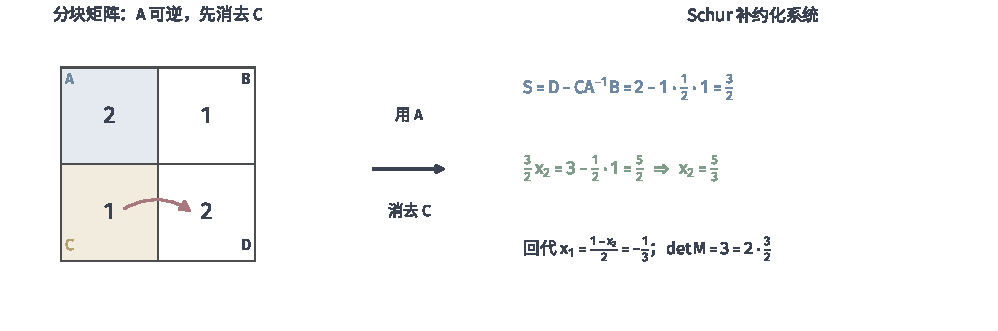
\includegraphics[width=168.998mm]{figures/01-mathematical-preliminaries-upper/02-linear-spaces/matplotlib/ls-schur-block-elimination/ls-schur-block-elimination.pdf}
  \caption{Schur 补的 2×2 分块消元。左：$\bm M=\left[\begin{smallmatrix}2&1\\1&2\end{smallmatrix}\right]$
  按左上块$\bm A=2$分块，先由第一行表出$x_1=(1-x_2)/2$；右：代入第二行后右下角残留
  Schur补$\bm S=3/2$，约化得$x_2=5/3$、回代$x_1=-1/3$，且$\det\bm M=2\cdot3/2=3$。
  解析式教学构造。}
  \label{fig:ls-schur-block-elimination}
\end{figure*}

下面把这一操作写成块记号。

把未知量分成两块，设
$\bm M=\left[\begin{smallmatrix}\bm A&\bm B\\\bm C&\bm D\end{smallmatrix}\right]$，
$\bm A\in\mathbb R^{p\times p}$可逆，右端$(\bm f^\top,\bm g^\top)^\top$。
第一组方程$\bm A\bm x+\bm B\bm y=\bm f$先把$\bm x=\bm A^{-1}(\bm f-\bm B\bm y)$
用$\bm y$表示，再代入第二组消去$\bm x$。典型来源是二部结构：全局参数块与各局部
块相连、局部块之间不直接相连，先分别消去各局部块，只剩全局块的小系统。

\paragraph{Schur补与约化系统}

\term{Schur补}（Schur complement）定义为
$\bm S=\bm D-\bm C\bm A^{-1}\bm B$。
\label{def:matrix-analysis-schur-complement}
代入第二组得到约化系统
\begin{equation}
 \bm S\bm y=\bm g-\bm C\bm A^{-1}\bm f,
 \label{eq:matrix-analysis-schur-complement}
\end{equation}
矩阵形式为
$\left[\begin{smallmatrix}\bm I&\bm0\\-\bm C\bm A^{-1}&\bm I\end{smallmatrix}\right]
\bm M=\left[\begin{smallmatrix}\bm A&\bm B\\\bm0&\bm S\end{smallmatrix}\right]$，
即左边乘一个单位下三角消去块左下角，把$\bm M$化成块上三角。在$\bm A$可逆
前提下，$\bm M$可逆当且仅当$\bm S$可逆，且$\det\bm M=\det\bm A\det\bm S$。
例如$\bm M=\left[\begin{smallmatrix}2&1\\1&2\end{smallmatrix}\right]$，
取$\bm A=2$、$\bm B=\bm C=1$、$\bm D=2$，则$\bm S=2-1/2=3/2$，
$\det\bm M=3=2\cdot3/2$，约化$3y/2=g-f/2$解出$y$后回代$x=(f-y)/2$。

解出$\bm y$后回代$\bm x=\bm A^{-1}(\bm f-\bm B\bm y)$。
逆通过求解$\bm A\bm Z=\bm B$、$\bm A\bm x=\bm f$来应用，不为套公式先形成整个
逆矩阵。需要时块逆为
\begin{equation}
 \bm M^{-1}=
 \begin{bmatrix}
  \bm A^{-1}+\bm A^{-1}\bm B\bm S^{-1}\bm C\bm A^{-1}
  &-\bm A^{-1}\bm B\bm S^{-1}\\
  -\bm S^{-1}\bm C\bm A^{-1}&\bm S^{-1}
 \end{bmatrix}.
 \label{eq:matrix-analysis-block-inverse}
\end{equation}
回代后必须代回原两块方程核验，约化系统相容不自动保证原方程每块满足。

$\bm M$对称时$\bm C=\bm B^\top$。配方给出
\begin{equation}
 \begin{bmatrix}\bm x\\\bm y\end{bmatrix}^{\top}
 \bm M\begin{bmatrix}\bm x\\\bm y\end{bmatrix}
 =(\bm x+\bm A^{-1}\bm B\bm y)^\top
 \bm A(\bm x+\bm A^{-1}\bm B\bm y)+\bm y^\top\bm S\bm y.
\end{equation}
右边两项分别为$\bm A$、$\bm S$的二次型。因此$\bm A\succ0$时
\begin{equation}
 \bm M\succ0\quad\Longleftrightarrow\quad
 \bm D-\bm B^\top\bm A^{-1}\bm B\succ0.
 \label{eq:matrix-analysis-schur-positive-definite}
\end{equation}
必要性可取$\bm x=-\bm A^{-1}\bm B\bm y$使第一项归零，只剩$\bm y^\top\bm S\bm y$
须对所有$\bm y$为正；充分性来自两项非负且不能同时为零（$\bm A$正定）。

对称正定等价于各阶顺序主子式为正，这正是逐块配方的主元；配方每步剩余矩阵正定，
故主元严格为正。半正定不能机械把严格不等号改为非严格，零主元对应真实退化，
主子式判据需另行处理零空间，不能套用正定除法；负主元（不定）则由LDL$^{\top}$
的块对角承接，不属Cholesky范围。

$\bm A$本身可能奇异，不能直接把$\bm A^{-1}$换成伪逆而不加条件；
需要$\operatorname{range}(\bm B)\subseteq\operatorname{range}(\bm A)$等值域条件
保证消去可行，以及伪逆版本的Schur补，再核验零空间是否留下自由参数。
不满足值域条件时，第一组方程$\bm A\bm x=\bm f-\bm B\bm y$对某些$\bm y$无解，
分块消元不能进行。

矩阵由$\bm A$变为$\bm A+\bm U\bm C\bm V^\top$，新增耦合只经过$k$个中间坐标
（$k$通常远小于$d$）。引入辅助未知量$\bm z=\bm V^\top\bm x$，把大系统换成$k$阶
小系统加已有$\bm A$的求解器，避免对$d$阶新矩阵重新分解；这是精确改变矩阵，不是
近似压缩，新矩阵与旧矩阵逐项不同。适用前提是旧求解器仍可用（$\bm A$可逆或已存
因子），$k$很小使小系统值得单独求解。

\paragraph{Woodbury恒等式与小系统}

设$\bm A$、$\bm C$与
$\bm S=\bm C^{-1}+\bm V^\top\bm A^{-1}\bm U$均可逆，按两种顺序消元同一块矩阵，
比较左上块得\term{Woodbury恒等式}
\begin{equation}
 (\bm A+\bm U\bm C\bm V^\top)^{-1}
 =\bm A^{-1}-\bm A^{-1}\bm U
 (\bm C^{-1}+\bm V^\top\bm A^{-1}\bm U)^{-1}
 \bm V^\top\bm A^{-1}.
 \label{eq:matrix-analysis-woodbury}
\end{equation}
取$\bm C=\bm I$时只需$\bm A$与$\bm I+\bm V^\top\bm A^{-1}\bm U$可逆，
无须对矩形$\bm U,\bm V$假定逆；实现为
$(\bm I+\bm V^\top\bm A^{-1}\bm U)\bm z=\bm V^\top\bm A^{-1}\bm b$，
再$\bm x=\bm A^{-1}(\bm b-\bm U\bm z)$。先消$\bm A$得小系统$\bm S$，
先消$\bm C^{-1}$得更新矩阵，两种消元左上块比较即得恒等式。

$k=1$时得Sherman--Morrison公式
$(\bm A+\bm u\bm v^\top)^{-1}
=\bm A^{-1}-\dfrac{\bm A^{-1}\bm u\bm v^\top\bm A^{-1}}
{1+\bm v^\top\bm A^{-1}\bm u}$，要求$1+\bm v^\top\bm A^{-1}\bm u\neq0$。
同一块行列式的两种消元给出
$\det(\bm A+\bm U\bm C\bm V^\top)
=\det\bm A\det\bm C\det\bm S$；行列式恒等式在小系统奇异时仍可能成立，
求逆公式则不能使用。例如$\bm A=\operatorname{diag}(2,3)$、
$\bm u=\bm v=(1,1)^\top$、$\bm b=(1,0)^\top$，直接解
$\left[\begin{smallmatrix}3&1\\1&4\end{smallmatrix}\right]\bm x=\bm b$
得$\bm x=(4/11,-1/11)^\top$，更新公式的标量
$1+\bm u^\top\bm A^{-1}\bm u=1+1/2+1/3=11/6$，代回同解，
行列式为$6\times11/6=11$。原分解已存在时，求$\bm A^{-1}\bm U$只需$k$次
三角求解；低秩更新精确改变矩阵，不是后文的低秩压缩任务，小系统接近奇异时公式
仍可能敏感。

\subsection{定常迭代法}
\label{sec:ls-stationary-iterations}
\label{sec:linear-algebra-stationary-splitting}

稀疏方程的一行往往只连接几个未知量，反复按行校正可以避免全局分解。
定常迭代每轮使用相同的校正规则；本节说明规则能否执行、怎样更新与核验，
收敛速率与暂态行为由后续收敛章节分析。

\subsubsection{矩阵分裂}

从近似解$\bm x^{(t)}$出发，定义当前残差
\begin{equation}
 \bm r^{(t)}=\bm b-\bm A\bm x^{(t)},
\end{equation}
它记录尚未消除的输出差距：$\bm r^{(t)}=\bm0$即精确解，否则方程要求再施加
$\bm A$把剩余差距补回。定常迭代不从零重建解，而只在当前近似上施加一轮校正，
因此每一步先有当前近似、才有要校正的残差。

把系数矩阵拆成$\bm A=\bm M-\bm N$，其中$\bm M$可逆且容易求解
（对角、三角、块对角或局部小系统），$\bm N$收集留给下一轮处理的耦合。
方程$\bm A\bm x=\bm b$改写为$\bm M\bm x=\bm N\bm x+\bm b$：把容易求解的
$\bm M$留在左端，难处理的耦合$\bm N\bm x$先用上一轮的值代入。这样每轮不必解
原系统，只解一个关于校正量的易解方程。分裂不是唯一的，同一$\bm A$可取不同
$\bm M$，直接决定每轮是否可执行、是否收敛；收敛性判据由后续收敛章节给出，
本节只保证方程可逐步更新。

\paragraph{残差校正的迭代公式}

定常迭代格式为
\begin{equation}
 \bm M\bm x^{(t+1)}=\bm N\bm x^{(t)}+\bm b,\qquad
 \bm x^{(t+1)}=\bm x^{(t)}+\bm M^{-1}\bm r^{(t)}.
 \label{eq:ls-stationary-splitting-form}
\end{equation}
第二式由$\bm M(\bm x^{(t+1)}-\bm x^{(t)})=\bm b-(\bm M-\bm N)\bm x^{(t)}
=\bm b-\bm A\bm x^{(t)}=\bm r^{(t)}$得到，校正量$\Delta\bm x=\bm M^{-1}\bm r^{(t)}$
正是“用易解的$\bm M$把当前残差反推成一次位移”。实现时只求
$\bm M\bm z=\bm r^{(t)}$再$\bm x^{(t+1)}=\bm x^{(t)}+\bm z$，不形成$\bm M^{-1}$；
形成逆矩阵既无必要，又会丢失$\bm M$容易求解的三角或对角结构。

设$\bm x_*$为精确解，由$\bm A\bm x_*=\bm b$与分裂$\bm A=\bm M-\bm N$，
误差$\bm e^{(t)}=\bm x^{(t)}-\bm x_*$满足
$\bm M\bm e^{(t+1)}=\bm N\bm e^{(t)}$，即
\begin{equation}
 \bm e^{(t+1)}=\bm T\bm e^{(t)},\qquad \bm T=\bm M^{-1}\bm N,
\end{equation}
$\bm T$称为误差传播矩阵。同一$\bm T$描述一轮后误差怎样被放大或缩小；对所有初值
收敛到$\bm x_*$等价于谱半径$\rho(\bm T)<1$。这一判据的证明、Jordan块的几何
衰减与速率估计归后续收敛章节，本节只指出：“能逐行更新”本身不是收敛证明，
$\bm T$的谱条件必须另行检查。

停止时复核原方程真实残差$\bm b-\bm A\bm x^{(t)}$，而不是递推中间量。
残差小不等于参数准确（条件数放大由后续章节说明），二者分开报告：先重算
$\bm r=\bm b-\bm A\bm x^{(t)}$，再按右端尺度归一判断是否达到容限。

\subsubsection{Richardson迭代}

取$\bm M=(1/\omega)\bm I$，即把易解算子取成标量恒等矩阵，校正方向就是残差
本身：每步沿$\bm r^{(t)}$移动$\omega$倍。这是最简单的定常迭代，不需要解任何
子系统，也是理解“用矩阵作用反复修正”的起点；$\omega$是唯一可调参数。

\paragraph{Richardson更新公式}

\term{Richardson迭代}（Richardson iteration）为
\begin{equation}
 \bm x^{(t+1)}=\bm x^{(t)}+\omega\bm r^{(t)},\qquad
 \bm r^{(t+1)}=(\bm I-\omega\bm A)\bm r^{(t)}.
 \label{eq:ls-richardson}
\end{equation}
第二式把残差递推单独写出：$\bm r^{(t+1)}=\bm b-\bm A(\bm x^{(t)}+\omega\bm r^{(t)})
=\bm r^{(t)}-\omega\bm A\bm r^{(t)}$。它能否收敛取决于$\omega$与$\bm A$，
不能只因每步使用了残差便认定有效。

对称正定时，可执行的充分步长区间为$0<\omega<2/\lVert\bm A\rVert_2$，
其中$\lVert\bm A\rVert_2$是算子范数尺度（由5.5节的极值工具给出上界）；
该区间只保证$\lVert\bm I-\omega\bm A\rVert_2<1$，是充分条件而非精确最优步长。
逐特征方向把残差乘以$1-\omega\lambda_i$的分解论证依赖6.3节才建立的
实对称正交特征基，本节只作前向预告，最优步长与收敛速度的证明留第7章。
一般可逆矩阵不保证存在可用的正步长，不能在谱坐标建立前把特征方向
当作当前前提；负特征值或复谱对应的方向可能被放大。

每步一次矩阵向量乘法$\bm A\bm x^{(t)}$与若干向量加法，不需要读取矩阵全部元素，
也不形成任何因子；这使它适合只能提供矩阵作用子程序的场景（黑箱算子），
但单步校正通常过慢，实际问题中多与预条件配合。$\omega$选错时该步甚至放大残差，
故步长约束是可执行前提而非优化细节。

每步重算$\bm r^{(t+1)}=\bm b-\bm A\bm x^{(t+1)}$核验，不使用递推中间量；
代价为一次矩阵作用加线性量级的向量运算，存储只需当前近似、残差和更新量三个向量。
步长$\omega$越界时残差可能回升，故每步残差是判断是否继续的直接依据。

\subsubsection{Jacobi迭代}

按第$i$行方程单独解出$x_i$：
\begin{equation}
 x_i=\frac{b_i-\sum_{j\neq i}a_{i,j}x_j}{a_{i,i}}.
\end{equation}
这一行把$x_i$用其余未知量表示，是把全局方程拆成逐行校正的起点；前提是
$a_{i,i}\neq0$，否则该行无法单独解出。

\paragraph{旧值替代与并行更新}

\term{Jacobi迭代}（Jacobi iteration）一轮内全部使用上一轮的旧值$\bm x^{(t)}$，
各行互不引用本轮新值，因此可以同时更新：
\begin{equation}
 x_i^{(t+1)}=\frac{b_i-\sum_{j\neq i}a_{i,j}x_j^{(t)}}{a_{i,i}}.
\end{equation}
旧值替代保证一轮内所有右端已知，天然适合并行；代价是同一轮内不利用刚算出的
改进信息。

记$\bm A=\bm D-\bm L-\bm U$，$\bm D$为对角部分，$\bm L,\bm U$分别为严格下、上
三角部分的相反数（故$\bm D-\bm L-\bm U$恰为$\bm A$）。Jacobi取$\bm M=\bm D$，
迭代矩阵
\begin{equation}
 \bm T_J=\bm D^{-1}(\bm L+\bm U).
\end{equation}
$\bm D$可逆时$\bm D^{-1}$只是各对角元取倒数，应用代价为线性量级。

每一步要求$a_{i,i}\neq0$；对角元为零时该行无法单独解出$x_i$，需先行列重排把
非零元换到对角，不能作除数。重排后仍须复核新对角非零；若整行只含零而右端非零，
那是相容性矛盾（无解），与对角可执行性是两件事。

若各行严格对角占优，即
\begin{equation}
 q=\max_i\frac{\sum_{j\neq i}|a_{i,j}|}{|a_{i,i}|}<1,
\end{equation}
则$\lVert\bm e^{(t+1)}\rVert_\infty\leq q\lVert\bm e^{(t)}\rVert_\infty$：把上式
代入误差递推，第$i$个新误差由旧各误差线性组合，系数和不超过$q$，故无穷范数每轮
压缩$q$倍。这是充分而非必要条件，不满足也可能收敛。对称正定也不保证Jacobi收敛：
例如对角元为$1$、非对角元均为$0.9$的三阶矩阵，特征值为$2.8,0.1,0.1$，虽正定，
Jacobi迭代矩阵却有特征值$1.8$（其余两个为$-0.9$），$|1.8|>1$，一般初值会发散。

每步按非零元数读取局部系数，各行无数据依赖，适合并行；停止前重算原系统残差
核验。每轮一次矩阵作用量级的工作，存储为当前与上一轮两个向量（因旧值须保留供
整轮同时读取）。Jacobi不利用本轮新值，这正是它可并行却通常慢于GS的代价。

\subsubsection{Gauss--Seidel迭代}

\term{Gauss--Seidel迭代}（Gauss--Seidel iteration）按$i=1,\ldots,d$的次序，
立即使用本轮刚算出的新值：第$i$行校正时，$j<i$的未知量已用本轮新值，$j>i$
仍用上一轮旧值。与Jacobi的差别只在“读新值还是旧值”，却改变了迭代矩阵与
收敛行为。

\paragraph{顺序更新公式}

\begin{equation}
 x_i^{(t+1)}=
 \frac{b_i-\sum_{j<i}a_{i,j}x_j^{(t+1)}
             -\sum_{j>i}a_{i,j}x_j^{(t)}}{a_{i,i}}.
\end{equation}
先求和的$j<i$项用新值、$j>i$项用旧值，逐行顺扫完成一轮；公式结构与Jacobi
相同，只是代入值的新旧不同。

取$\bm M=\bm D-\bm L$（对角加取相反数后的严格下三角），每轮相当于解一次下三角
系统$\bm M\bm x^{(t+1)}=\bm b+\bm U\bm x^{(t)}$，按$i=1,\ldots,d$顺序前代即得
更新；迭代矩阵
\begin{equation}
 \bm T_{GS}=(\bm D-\bm L)^{-1}\bm U.
\end{equation}
下三角前代无需求逆，逐行代入即可。

扫描顺序决定数据依赖，也改变迭代矩阵$\bm T_{GS}$；未知量重排后方法行为不同，
这不是可忽略的实现细节。同一矩阵按不同次序扫描，一轮压缩效果可能明显变化；
带宽小、依赖局部的排序通常更利于顺序传播改进，但最优排序的定量比较归后续章节。

严格对角占优时Gauss--Seidel与Jacobi有同一上界$q$：沿扫描顺序归纳，已更新误差
不超过旧误差最大值，代回当前行后进一步不超过$q$倍。对称正定时Gauss--Seidel
可用（能量下降的完整证明留待后续收敛章节），但该保证不传给Jacobi——正定只保证
GS类顺序扫描的能量单调，不保证并行的Jacobi。

以$\bm A=\left[\begin{smallmatrix}4&-1\\-1&3\end{smallmatrix}\right]$、$\bm b=(1,2)^\top$、
零初值复核一轮：
\begin{equation*}
 \text{Jacobi}=(1/4,2/3)^\top,\qquad
 \text{Gauss--Seidel}=(1/4,3/4)^\top,
\end{equation*}
二者极限均为$(5/11,9/11)^\top$。Gauss--Seidel 第二行立即读取已更新的$1/4$，
故第一轮数值与存储依赖已与 Jacobi 不同。每轮一次顺序扫描，停止前重算原系统残差。

\subsubsection{SOR迭代}

先用本轮可用值算出Gauss--Seidel候选$\widetilde{x}_i$，再把实际更新写成旧值与
候选值的加权校正，而不是一步跳到候选：这引入一个调节幅度的参数，便于在过冲与
欠校之间选择，也是SOR相对GS的唯一改动。$\omega=1$时候选即实际更新，SOR退回GS。

\paragraph{松弛参数与逐行更新}

\term{逐次超松弛}（successive over-relaxation, SOR）令
\begin{equation}
 x_i^{(t+1)}=(1-\omega)x_i^{(t)}+\omega\widetilde{x}_i.
\end{equation}
$\omega=1$退回Gauss--Seidel；$0<\omega<1$减小校正（欠松弛），
$\omega>1$越过候选值（超松弛）。$\omega$是逐行共用的标量参数。

\begin{equation}
 (\bm D-\omega\bm L)\bm x^{(t+1)}
 =\bigl((1-\omega)\bm D+\omega\bm U\bigr)\bm x^{(t)}+\omega\bm b.
 \label{eq:linear-algebra-sor-splitting}
\end{equation}
左端$\bm D-\omega\bm L$为下三角，可顺序前代求解；右端收集旧值与$\omega\bm b$。

对称正定时充分范围为$0<\omega<2$。固定第$i$坐标展开二次能量
$\phi(\bm x)=\tfrac12\bm x^\top\bm A\bm x-\bm b^\top\bm x$，记更新前该行残差$r_i$，
$\Delta x_i=\omega r_i/a_{i,i}$，单步能量增量为
\begin{equation}
 \phi(\bm x+\Delta x_i\bm e_i)-\phi(\bm x)
 =-\frac{\omega(2-\omega)}{2a_{i,i}}r_i^2.
\end{equation}
正定性保证$a_{i,i}>0$与能量有下界；固定$0<\omega<2$使$\omega(2-\omega)>0$，
每轮各坐标校正趋零，完整收敛证明留待后续章节。

$\omega$超出$(0,2)$时$\omega(2-\omega)<0$，校正方向反转、能量上升；参数大并不
保证更快，最优$\omega$依赖矩阵结构，无条件宣称超松弛更快超出本节保证。
$\omega=0$停在旧值不更新，$\omega=2$恰使能量增量项为零、无改进，二者均非
有效步长。

每轮一次顺序扫描，工作量与Gauss--Seidel同级，仅多一次标量加权；停止前重算原
系统残差$\bm b-\bm A\bm x^{(t)}$，递推残差不作为停止依据。$\omega$固定后每步
成本不变，存储与GS相同，不需要额外向量。

\subsubsection{分块迭代}

把未知量分成若干块$\bm x=(\bm x_1^\top,\ldots,\bm x_s^\top)^\top$，按块隔离方程，
单变量规则推广为块级校正：每块内部允许耦合（块内不必再拆），块间连接留给迭代；
分组可对应物理区域、网格分块或变量类型，分组越细块内越好解、块间迭代越多。
例如把网格按区域分成若干块，块内用直接法一次解完，块边界的耦合由迭代逐步消除。

块Jacobi取块对角分裂$\bm M=\operatorname{diag}(\bm A_{11},\ldots,\bm A_{ss})$，
各块用块内直接法独立求解、同时更新，块间用旧块值代入，
对应单变量Jacobi的并行结构：一轮内各块右端已知，互不等待，适合分块并行。

块Gauss--Seidel按块顺序$1,\ldots,s$立即使用已解出的新块值，前一块新值进入后一块
的右端，对应单变量GS的顺序扫描；块间有计算依赖，不能并行，但每轮通常利用了更新
信息。块SOR再在块级引入松弛参数，与单变量SOR平行。

每个对角块必须可逆或可解；局部块求解本身可以调用前面的直接法（LU、Cholesky或
QR），块分裂因此把大问题换成若干可独立处理的小系统。某块奇异时不能作块分裂的
主元，需重新分组或转入相容性判断，不能把块逆直接套公式。

分组改变每轮子问题成本与块间耦合：块切得大，块内求解贵而耦合弱、迭代少；块切得小，
块内便宜而耦合强、迭代多。收敛仍需检查相应块迭代矩阵，证明归后续收敛章节。

\subsection{预条件的构造与应用}
\label{sec:ls-preconditioning}

预条件为迭代配置一个容易应用的辅助求解器，把原方程改写成更适合校正的等价系统。
本节只构造与应用预条件，条件数改善与收敛速率归后续章节。

\subsubsection{等价系统与残差}

选可逆且易解的$\bm M$近似$\bm A$：$\bm M\bm z=\bm r$比$\bm A\bm x=\bm b$容易
（对角、三角、块对角或不完全因子）。预条件不改变精确解，但改变迭代读取的残差与
搜索空间，使校正方向更接近真实解方向。$\bm M=\bm A$虽使变换后系统简单，却已
付出原求解成本，失去预条件意义；$\bm M$必须“既接近$\bm A$又容易解”，二者权衡。

\term{左预条件}解$\bm M^{-1}\bm A\bm x=\bm M^{-1}\bm b$，迭代最小化的是变换后
残差$\bm M^{-1}(\bm b-\bm A\bm x)$，不是原始残差；实现只求$\bm M\bm z=\bm r$，
不显式形成$\bm M^{-1}$。停止时看到的小残差是变换后口径，必须换回原系统残差才能
判断原方程是否满足。

\term{右预条件}令$\bm x=\bm M^{-1}\bm z$，解$\bm A\bm M^{-1}\bm z=\bm b$；
搜索方向在$\bm z$空间，求得$\bm z$后须经$\bm M^{-1}$映回$\bm x$。左、右预条件
不改变精确解，但改变被最小化的残差口径：左预条件改变残差尺度，右预条件改变搜索
方向所在空间。

CG所需的对称结构要求$\bm M$对称正定，$\bm M=\bm L\bm L^\top$时等价对称系统为
$\bm L^{-1}\bm A\bm L^{-\top}\bm z=\bm L^{-1}\bm b$。一般非对称的
$\bm M^{-1}\bm A$不在标准欧氏内积下对称，不能配任意预条件器继承CG的正分母与
能量论证。

实现只求$\bm M\bm z=\bm r$，利用$\bm M$的三角或对角结构逐行代入，不保存也不
显式形成$\bm M^{-1}$；显式求逆会破坏易解结构（三角因子变稠密）并增加存储，
也丢失逐行代入的廉价路径。“近似逆”只是名称，实现仍是解一个易解系统。

\subsubsection{基于局部结构的预条件}

\term{对角预条件}取$\bm M=\operatorname{diag}(\bm A)$，只校正各方向尺度，把
量级悬殊的对角元拉平；构造与应用最便宜，每个$z_i=r_i/a_{ii}$一次除法，不处理
任何非对角耦合。对角元为零时无法作除数，需先重排或改用块对角；它只对方向尺度
失衡有效，对强耦合帮助有限。

块对角预条件保留块内耦合、忽略块间连接；块内用小直接法（LU 或 Cholesky）求解，
代价高于对角预条件但保留了局部结构，块间耦合由迭代逐步消除。块的取法与
6.2.4.6 分块迭代一致，块内可逆是前提。

由SOR的一轮前向扫描（$i=1,\ldots,d$）再配一轮对称后向扫描（$i=d,\ldots,1$），
组合成\term{SSOR}（对称SOR）预条件；两次扫描互为反向，组合后的算子本身对称
正定，可用于PCG。它不需要额外分解，只复用SOR的三角递推，$\omega$沿用SOR参数。
SSOR应用时先前代（前向扫描，从小到大）再回代（后向扫描，从大到小），次序与构造
一致；每步成本为两次三角求解，与一轮SOR同级。前向或后向单独使用只得到非对称
算子，两轮对称组合才恢复正定性，顺序不可颠倒或省略。

预条件保留的局部耦合越多，每次应用越贵，构造成本也越高，需与迭代次数一起权衡，
不能只看构造是否便宜。对角最便宜但改善小，块对角/SSOR/ILU逐次更贵但每步压缩
更多，三者乘上迭代次数才是总账。

\subsubsection{基于不完全分解的预条件}

完整LU或Cholesky的填充使稀疏因子退化为准稠密，建立时间与存储都可能不可接受，
这正是不完全分解要避免的；填充位置取决于行列排序，同一矩阵不同排序填充量差别
很大。规则网格的完整分解可能填满原零区，而保留原模式的不完全分解保持稀疏。

\term{不完全分解}（incomplete factorization）规定保留的非零模式（pattern，通常取
原矩阵非零位置，或叠加若干层邻接），消元中落到模式外的填充项直接舍弃，因子保持
稀疏；舍弃位置不补回，误差由迭代逐步消除。模式选得越宽越接近完整分解、越贵，
选得越窄越便宜但预条件改善越小。

不完全Cholesky（IC）对对称正定矩阵按与完整Cholesky相同的递推构造，但只写回保留
位置；遇到非正主元（舍弃使剩余不再严格正定）需按规则修正（对角平移，把主元抬高
到正阈值），不能照搬完整Cholesky的开方。修正改变了预条件，不再是原矩阵的精确
因子。

不完全LU（ILU）对一般矩阵按保留模式消元，应用时两次三角求解（前代、回代），
不追求因子精确等于$\bm A$，舍弃项由迭代补偿。ILU不要求对称或正定，适用面比IC
宽，但同样可能出现零主元，需要部分主元或修正规则。

舍弃可能造成零主元或不稳定，需要对角修正、部分主元等规则；修正改变了预条件本身，
失效条件与敏感性（修正量多大、何时改回直接法）留后续章节说明。零主元不能硬除，
应停止并换模式或换方法。

\subsubsection{代价与效果}

预条件总成本必须分别计入构造（一次：分解或建立$\bm M$）与每次辅助求解（每步迭代
都调用$\bm M\bm z=\bm r$），二者不可只报其一；便宜的构造可能伴随昂贵的每步应用，
例如ILU建立一次但每步两次三角求解，而对角预条件建立几乎免费、每步仅除法。

用总求解成本而非单步速度评价：便宜预条件可能需要更多迭代，贵预条件可能减少步数，
二者相乘（构造成本$+$每步成本$\times$迭代次数）才是比较口径。条件数改善使步数
下降的定量估计归后续收敛章节，本节只要求把两类成本同时列出。

固定矩阵、多个右端时，一次性构造成本（分解或预条件建立）被各列摊销，每列只承担
自己的辅助求解与迭代；逐列迭代也要分别报告真实残差，不能用一列的进展代替另一列。
若矩阵本身改变，摊销前提失效，须重新建立。

左预条件迭代读取$\bm M^{-1}\bm r$，停止判断必须回到原始残差
$\bm b-\bm A\bm x$，不能把变换后残差直接当作原方程误差；两者尺度可能相差很大，
$\bm M^{-1}\bm r$小不代表$\bm r$小。报告结果时同时给出两种残差，停止阈值只对
原始残差设定。

按目标精度、可访问数据与存储预算选择：高精度且矩阵可整体获得时优先直接法，
只能提供矩阵作用或规模极大时选Krylov并配预条件。结果始终以原系统残差核验，
并复核所选方法的前提（可逆、正定、非零对角、分母非零）是否满足。

\subsection{Krylov子空间迭代法}
\label{sec:ls-krylov-methods}
\label{sec:ch06-iterative-solvers}

当完整分解产生过多填充，或矩阵本身只以“输入向量、返回乘积”的程序给出时，
无法再显式读取并存储因子。消元（LU/Cholesky）需要改动矩阵元素，而稀疏矩阵中
大量原本为零的位置会在消元过程中被填入非零数（填充，见6.2.3.1），可能从
“只占很少存储”退化成近乎稠密；更极端时矩阵大到根本无法整体存储，只提供一个
给定向量就返回$\bm A\bm v$的子程序。此时只能反复利用矩阵—向量乘法逐步逼近解。
本节说明候选空间怎样生成、在空间内按什么准则挑选系数、怎样停止核验；
收敛速度、多项式逼近与误差估计由后续收敛章节处理。

\subsubsection{子空间构造}

先看最小的生成过程。取$\bm A=\left[\begin{smallmatrix}2&1\\1&3\end{smallmatrix}\right]$、
$\bm r_0=(1,0)^\top$，反复作用得$\bm A\bm r_0=(2,1)^\top$、
$\bm A^2\bm r_0=(5,5)^\top$。前两个方向$(1,0)^\top$与$(2,1)^\top$已经张满
$\mathbb R^2$，第三个$(5,5)^\top=5(2,1)^\top-5(1,0)^\top$落在其中，不再扩大空间。
可见从一个残差出发、只允许反复乘$\bm A$，候选方向就是这条幂链及其张成空间；
维数有限时它迟早停止增长。下面把它写成一般形式。

从初值$\bm x_0$出发，先定义当前残差$\bm r_0=\bm b-\bm A\bm x_0$，它记录
尚未消除的输出差距，也是一切候选方向的起点。每一步只允许使用一次矩阵作用
$\bm v\mapsto\bm A\bm v$，因此新方向只能由残差反复被$\bm A$作用得到：
$\bm r_0,\bm A\bm r_0,\bm A^2\bm r_0,\ldots$。这一限制不是任意约定：当矩阵
不可整体获得时，除了$\bm A$作用之外没有别的算子可用，全部候选方向都必须由
这条生成链产生。

\paragraph{Krylov空间中的校正表示}

由生成链张成的空间称为\term{Krylov子空间}（Krylov subspace）
\begin{equation}
 \mathcal K_k(\bm A,\bm r_0)
 =\operatorname{span}\{\bm r_0,\bm A\bm r_0,\ldots,\bm A^{k-1}\bm r_0\}.
\end{equation}
把校正量写成该空间的组合
\begin{equation}
 \bm x_k=\bm x_0+\sum_{j=0}^{k-1}\alpha_j\bm A^j\bm r_0,
\end{equation}
任务便从“找一个$d$维向量”缩小为“挑$k$个组合系数”。误差$\bm e_k=\bm x_k-\bm x_*$
与校正量沿同一空间推进：令$\bm e_0=\bm x_0-\bm x_*$，由$\bm x_k$的表示直接相减得
\begin{equation}
 \bm e_k=\bm e_0+\sum_{j=0}^{k-1}\alpha_j\bm A^j\bm r_0.
\end{equation}
再用$\bm r_0=\bm b-\bm A\bm x_0=-\bm A\bm e_0$，即得
\begin{equation}
 \bm e_k=\left(\bm I-\sum_{j=0}^{k-1}\alpha_j\bm A^{j+1}\right)\bm e_0,
\end{equation}
所以误差也落在$\bm e_0$被$\bm A$反复作用的同一幂链上。梯度法也可能生成这种空间，故梯度法与
Krylov方法不是互斥类别；这里只按“空间由矩阵幂链生成”组织。

扩基只保证候选集合包含更多方向；在空间内按能量误差、残差或其他准则挑系数，
是独立的第二步，二者不能混为一谈。把候选解限制在$\bm x_0+\mathcal K_k$内后，
最优系数$\bm\alpha$由一个$k$阶小规模问题决定：CG在其中最小化能量误差，
MINRES/GMRES在其中最小化欧氏残差。规模$k$随步数增长，但每一步的小问题远小于
原$d$维系统。生成空间（扩基）与空间内优化（挑系数）分开陈述，正是为了避免把
“方向越来越多”误当成“解已经更好”。

\paragraph{Arnoldi正交扩基}

直接使用幂链$\bm A^j\bm r_0$作基会严重病态：相邻方向几乎重合，系数矩阵条件数
随$k$迅速恶化。\term{Arnoldi过程}每次计算$\bm w=\bm A\bm v_j$，依次减去
$h_{i,j}\bm v_i$（$h_{i,j}=\bm v_i^\top\bm w$），把$\bm w$对全部已存正交基
$\bm v_1,\ldots,\bm v_j$投影扣除，余量归一化得到$\bm v_{j+1}$。它建立正交基
$\bm V_k$，使$\bm A\bm V_k=\bm V_{k+1}\overline{\bm H}_k$，
$\overline{\bm H}_k$为$(k+1)\times k$上Hessenberg小矩阵（主对角线下第二条及
更低位置为零），记录矩阵在逐渐扩大的搜索空间中的作用。新向量依次对全部已存基
正交化，这也是GMRES扩基的同一机制。

\paragraph{对称作用与Lanczos短递推}

当$\bm A$实对称时，Hessenberg结构退化为对称三对角，不必把新向量对全部旧基
投影：\term{Lanczos短递推}只需相邻三个向量即可更新，$\bm A\bm V_k=\bm V_{k+1}\bm T_k$，
$\bm T_k$为对称三对角。短递推（Lanczos、CG、BiCGSTAB）只保留几个向量即可更新；
Arnoldi/GMRES保存全部正交基，二者是存储与步数之间的不同选择，不是优劣之分。
对称作用让三对角化成为可能，非对称方阵没有这条短递推。

校正量$\sum_j\alpha_j\bm A^j\bm r_0$等价于用多项式$p_k(\bm A)$作用于$\bm r_0$，
其中$p_k(0)=1$。残差$\bm r_k=\bm r_0-p_k(\bm A)\bm A\bm r_0=q_k(\bm A)\bm r_0$，
$q_k$为次数不超过$k$、常数项为1的多项式。在$\mathcal K_k$内选最优系数，就是选
这样一个多项式使目标（能量误差或残差范数）最小；这一多项式观点把各Krylov方法
统一到同一框架，但多项式逼近的质量与速度由后续收敛章节分析，本节只说明空间与
挑选准则如何建立。

若某步余量长度$h_{j+1,j}=0$，说明当前空间已是$\bm A$的不变子空间，应停止扩基，
不对零向量归一化。先检查空间中是否含解再停止：若$\bm A$可逆且$\bm r_0$属于
该不变空间，则精确校正量$\bm A^{-1}\bm r_0$也在其中，精确解属于当前仿射候选集
$\bm x_0+\mathcal K_j$；若$\bm A$奇异或空间不含解，则转入选解或最小二乘判断，
不能继续除以零。有限维下幂链至多$d$个方向线性无关，空间不会无限增长。

把$\mathcal K_k$正交化成$\bm V_k$后，原问题化为$k$阶小型最小二乘或三角问题；
小型QR直接回用上文6.1.3.1建立的工具（经济型QR、Givens旋转逐步更新），
每次只更新边界一行一列，无需解大的正规方程。具体地，Arnoldi关系
$\bm A\bm V_k=\bm V_{k+1}\overline{\bm H}_k$把残差写成正交基$\bm V_{k+1}$的线性
组合，因$\bm V_{k+1}$列正交，范数等于小矩阵$\overline{\bm H}_k$对应最小二乘问题的
残差范数，Givens旋转每步消去新增一行即可。递推中估计的残差（由小问题后向求解读出）
与真实残差在有限精度下可能分离，停止判断以重算的真实残差$\bm b-\bm A\bm x_k$为准。

\subsubsection{CG与PCG}
\label{sec:ch06-conjugate-gradient}

CG 不是通用迭代法，它只在三条前提同时满足时才能使用能量论证：
\begin{enumerate}
 \item 对称性$\bm A=\bm A^\top$：使梯度$\bm A\bm x-\bm b$对应一个二次目标。
 \item 正定性$\bm x^\top\bm A\bm x>0$（$\bm x\neq\bm0$）：使$\lVert\cdot\rVert_{\bm A}$
 为范数、一维步长分母$\bm p^\top\bm A\bm p>0$。
 \item 右端无限制：$\bm b$任意；不定或非对称$\bm A$应改用 MINRES/GMRES。
\end{enumerate}
满足时方程$\bm A\bm x=\bm b$等价于最小化二次目标
\begin{equation}
 \phi(\bm x)=\tfrac12\bm x^\top\bm A\bm x-\bm b^\top\bm x,
\end{equation}
其“梯度”为$\bm A\bm x-\bm b$（微积分名称在后续章节引入）。设$\bm x_*=\bm A^{-1}\bm b$
为精确解，$\bm e=\bm x-\bm x_*$，则
\begin{equation}
 \phi(\bm x)-\phi(\bm x_*)=\tfrac12\bm e^\top\bm A\bm e
 =\tfrac12\lVert\bm e\rVert_{\bm A}^2,
\end{equation}
即目标差就是能量误差平方的一半。正定性使$\lVert\cdot\rVert_{\bm A}$为范数，
故$\phi$有唯一极小点，且它正是方程的解；$\bm x^{(0)}+\mathcal K_k(\bm A,\bm r_0)$
中使能量误差最小的点，就是CG的候选。

\paragraph{共轭方向与互不干扰的校正}

沿方向$\bm p$精确一维最小化后，有$\bm p^\top\bm r=0$；再沿$\bm q$移动$s$，
残差变成$\bm r-s\bm A\bm q$。若$\bm p^\top\bm A\bm q=0$，新残差仍与$\bm p$
正交，先前沿$\bm p$达到的一阶最优条件便被保留。方向$\bm p_i,\bm p_j$满足
$\bm p_i^\top\bm A\bm p_j=0\ (i\neq j)$时称为\term{A共轭}（A-conjugate）。
需要的是$\bm A$共轭而非普通欧氏正交：普通正交只保证$\bm p^\top\bm q=0$，
不能保证$\bm p^\top\bm A\bm q=0$，沿$\bm q$移动仍可能破坏$\bm p$方向已完成的
最优。图~\ref{fig:vol1-add-linear-conjugate-directions}给出解析教学示例：
目标$\phi=\tfrac12(x_1^2+4x_2^2)$，从$(4,0)^\top$沿$\bm p=(1,1)^\top$
精确线搜索到$(3.2,-0.8)^\top$，再沿$\bm q=(-4,1)^\top$直达原点，
两方向满足$\bm p^\top\bm A\bm q=0$，第二步保持$\bm p$方向的最优。
\begin{figure}[!htb]
  \centering
  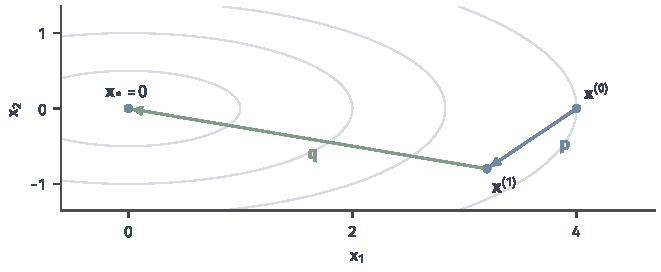
\includegraphics[width=112mm]{figures/01-mathematical-preliminaries-upper/02-linear-spaces/matplotlib/comprehension-additions/linear-conjugate-directions.pdf}
  \caption{共轭方向保留已完成的方向优化。目标为$\phi(\bm x)=\tfrac12(x_1^2+4x_2^2)$，
  灰线为等值线；从$(4,0)^\top$先沿$\bm p=(1,1)^\top$精确线搜索至$(3.2,-0.8)^\top$，
  再沿$\bm q=(-4,1)^\top$到达原点，两方向满足$\bm p^\top\bm A\bm q=0$。本图为解析教学示例。}
  \label{fig:vol1-add-linear-conjugate-directions}
\end{figure}

沿当前方向$\bm p_t$把$\phi$看作步长$\alpha$的一元函数
$\phi(\bm x_t+\alpha\bm p_t)$，展开后对$\alpha$求零点（一维最小化）得
\begin{equation}
 \alpha_t=\frac{\bm p_t^\top\bm r_t}{\bm p_t^\top\bm A\bm p_t}.
\end{equation}
分子是当前方向与残差的配对，分母是方向的能量长度。正定性保证分母
$\bm p_t^\top\bm A\bm p_t>0$，步长合法；若分子为零说明该方向已无改进，
不应再沿它移动。步长不是经验调节参数，而是这一一维最小化的唯一解。

\paragraph{残差正交与方向短递推}

\term{共轭梯度法}（conjugate gradient, CG）从$\bm p_0=\bm r_0$开始：
\begin{align}
 \alpha_t&=\frac{\bm r_t^\top\bm r_t}{\bm p_t^\top\bm A\bm p_t},&
 \bm x_{t+1}&=\bm x_t+\alpha_t\bm p_t,\\
 \bm r_{t+1}&=\bm r_t-\alpha_t\bm A\bm p_t,&
 \beta_t&=\frac{\bm r_{t+1}^\top\bm r_{t+1}}{\bm r_t^\top\bm r_t},\\
 \bm p_{t+1}&=\bm r_{t+1}+\beta_t\bm p_t.&
\end{align}
系数由归纳同时保证三件事：非零残差$\bm r_0,\ldots,\bm r_t$彼此正交；
方向$\bm p_0,\ldots,\bm p_t$彼此$\bm A$共轭；前$t+1$个残差与方向都张成
$\mathcal K_{t+1}$。$t=0$由$\bm p_0=\bm r_0$成立。线搜索使新残差与当前方向
正交；对更早的$j<t$，由$\bm A\bm p_j=(\bm r_j-\bm r_{j+1})/\alpha_j$属于
$\mathcal K_{t+1}$，新残差与之正交，故$\bm r_{t+1}\perp\mathcal K_{t+1}$。
只剩与$\bm p_t$共轭一项需要选$\beta_t$：由新旧残差正交得
$(\bm r_{t+1})^\top\bm A\bm p_t=-\lVert\bm r_{t+1}\rVert_2^2/\alpha_t$，
$(\bm p_t)^\top\bm A\bm p_t=\lVert\bm r_t\rVert_2^2/\alpha_t$，
取$\beta_t=\lVert\bm r_{t+1}\rVert_2^2/\lVert\bm r_t\rVert_2^2$后
$\bm p_{t+1}=\bm r_{t+1}+\beta_t\bm p_t$便与$\bm p_t$共轭，归纳闭合。
$\bm r_t^\top\bm r_t$出现在$\alpha_t$分子，正是因为$(\bm p_t)^\top\bm r_t
=\lVert\bm r_t\rVert_2^2$。

\paragraph{PCG的预条件残差}

\term{预条件共轭梯度}（preconditioned CG, PCG）以对称正定$\bm M$配置预条件，
等价变换系统为$\bm L^{-1}\bm A\bm L^{-\top}\bm z=\bm L^{-1}\bm b$（$\bm M=\bm L\bm L^\top$）。
实现时不解变换坐标，而是每步解$\bm M\bm z_t=\bm r_t$，这里的$\bm z_t$是
预处理后的残差而非变换坐标；初始方向也必须同步改为$\bm p_0=\bm z_0$，
不能只替换迭代中的系数。系数同步改变为
$\alpha_t=\bm r_t^\top\bm z_t/(\bm p_t^\top\bm A\bm p_t)$，
$\beta_t=\bm z_{t+1}^\top\bm r_{t+1}/(\bm z_t^\top\bm r_t)$，
$\bm p_{t+1}=\bm z_{t+1}+\beta_t\bm p_t$。直接把一般非对称左预条件矩阵当作
欧氏对称矩阵是不对的，非对称预条件器不能继承CG的正分母与能量论证。

正定性保证非零方向的$\bm p_t^\top\bm A\bm p_t>0$，分母合法。新残差为零即停止，
不再做含零分母的更新。各次方向更新保证$\bm x_k-\bm x_0\in\mathcal K_k$，
残差与$\mathcal K_k$正交正是该子空间内极小化的一阶条件，正定性又使其充分。
非零共轭方向必线性无关，因此精确算术下至多$d$步得零残差；有限精度下正交性
受损，不能把有限步结论当作实现保证，实际步数与停滞由后续章节说明。
可复算小例子：$\bm A=\operatorname{diag}(1,2)$、$\bm b=(1,1)^\top$、零初值。
第一步$\alpha_0=2/3$得$\bm x^{(1)}=(2/3,2/3)^\top$、
$\bm r^{(1)}=(1/3,-1/3)^\top$，$\beta_0=1/9$给
$\bm p^{(1)}=(4/9,-2/9)^\top$；第二步$\alpha_1=3/4$得
$\bm x^{(2)}=(1,1/2)^\top$，残差恰为零。

每步一次矩阵作用$\bm A\bm p_t$、若干内积（$\bm r_t^\top\bm r_t$、
$\bm p_t^\top\bm A\bm p_t$）与向量更新（$\bm x_{t+1}$、$\bm r_{t+1}$、$\bm p_{t+1}$），
额外存储$O(d)$个向量（当前解、残差、方向；PCG再加预处理残差$\bm z_t$），
不需要形成$\bm A^{-1}$或任何稠密因子。预条件作用、
内积与辅助求解$\bm M\bm z_t=\bm r_t$都计入每步成本；矩阵作用本身按$\bm A$的
非零结构计，稠密与稀疏差别显著。

\subsubsection{MINRES}

\paragraph{对称不定系统与残差目标}

矩阵仍实对称但不正定时，能量范数$\lVert\cdot\rVert_{\bm A}$与正分母失效，
CG的能量最小化论证不能沿用。\term{MINRES}（minimum residual）改在
$\mathcal K_k$中直接最小化原方程残差$\lVert\bm A\bm x-\bm b\rVert_2$，
不要求$\bm A$正定；对称不定性本身不导致不可解，只是不能继续使用CG的
正分母或能量范数论证。

沿用Lanczos短递推构造正交基$\bm V_k$，使
$\bm A\bm V_k=\bm V_{k+1}\bm T_k$，$\bm T_k$为对称三对角（对称使Hessenberg的
次对角与上对角相等，非对角非零项只剩相邻两条）。大系统被压成
逐步更新的小型三对角问题，短递推只需相邻三个向量、不需保存全部基；有限精度下
正交性逐渐损失，必要时重正交化会增加存储与计算。

候选$\bm x=\bm x_0+\bm V_k\bm y$的残差写成$\bm V_{k+1}(\beta\bm e_1-\bm T_k\bm y)$，
其中$\beta=\lVert\bm r_0\rVert_2$；由于$\bm V_{k+1}$列正交，问题化为
\begin{equation}
 \min_{\bm y}\lVert\beta\bm e_1-\bm T_k\bm y\rVert_2.
\end{equation}
这个小型最小二乘用上文的小型QR求解，三对角边界每次只更新一个角，
用Givens旋转逐步完成，无需解大的正规方程。

求得小问题系数$\bm y$后，由$\bm x_k=\bm x_0+\bm V_k\bm y$
恢复解向量；随$\bm V_k$逐列增长，$\bm y$与解都可递推更新，不必每步从头重组。
实现上通常不直接保存$\bm V_k$乘以完整$\bm y$，而是用递推形式更新解向量；
这与CG只保留几个向量不同，MINRES的三对角短递推保留基的投影关系，
恢复路径同样只依赖相邻几列。

预条件仍要求对称正定$\bm M$；投影在$\bm M$内积下进行，
解释的是$\bm M^{-1/2}$尺度下的残差，停止时仍须回到原始残差$\bm b-\bm A\bm x$
核验，不能把变换后残差当作原方程误差。对称不定$\bm A$配上对称正定
（SPD, symmetric positive definite）预条件后，短递推与
三对角结构保持；非对称$\bm M$会破坏三对角对称关系，不满足MINRES前提。

MINRES可扩展到对称奇异相容系统的最小二乘任务，
但一般不保证给出最小欧氏范数代表；它在核方向上的取值仍可能携带自由分量，
选解需另核，MINRES-QLP等变体（专门约束到零空间正交补）不在本节展开。
奇异系统须先判相容（6.2.1），不相容时残差最小化归后续最小二乘任务。

每步一次矩阵作用加少量向量更新，三对角短递推存储与$k$
无关（只需相邻几个向量）；停止以重算的真实原残差$\bm b-\bm A\bm x_k$核验，
递推估计残差在有限精度下可能分离。若 Lanczos 提前出现零余量，说明空间已不变，
应在当前小问题内取残差极小并停止，不对零向量归一化。

\subsubsection{GMRES}
\label{sec:ch06-gmres}

\paragraph{一般系统与Krylov残差目标}

对可逆的一般方阵（无对称性要求），\term{广义最小残差法}（generalized
minimal residual, GMRES）选择
\begin{equation}
 \bm x_k=\argmin_{\bm x\in\bm x_0+\mathcal K_k(\bm A,\bm r_0)}
 \lVert\bm b-\bm A\bm x\rVert_2.
\end{equation}
它放宽的是对称正定要求，不是完全取消结构条件：这里假设$\bm A$可逆；
方法也能用于其他方阵，但其解集与终止结论要另核。

令$\gamma=\lVert\bm r_0\rVert_2>0$，
$\bm v_1=\bm r_0/\gamma$。Arnoldi过程建立正交基$\bm V_k$，满足
$\bm A\bm V_k=\bm V_{k+1}\overline{\bm H}_k$，$\overline{\bm H}_k$为
$(k+1)\times k$上Hessenberg小矩阵。候选$\bm x=\bm x_0+\bm V_k\bm y$的残差为
$\bm V_{k+1}(\gamma\bm e_1-\overline{\bm H}_k\bm y)$，因$\bm V_{k+1}$列正交，
只需解小型最小二乘$\min_{\bm y}\lVert\gamma\bm e_1-\overline{\bm H}_k\bm y\rVert_2$。

小型问题用Givens旋转逐步更新小型QR（见上文Givens旋转），每步只消去
新进入的一行，最后由$\bm x_k=\bm x_0+\bm V_k\bm y$恢复。若第$k$步剩余
长度为零，关系改为$\bm A\bm V_k=\bm V_k\bm H_k$，小问题相应使用
$k\times k$矩阵$\bm H_k$，无需构造不存在的新基向量。可复算小例子：
$\bm A=[1\ 1;0\ 2]$、$\bm b=(0,1)^\top$、零初值。第一步候选$(0,t)^\top$，
残差$(-t,1-2t)^\top$，最小化$t^2+(1-2t)^2$得$t=2/5$，残差范数
$1/\sqrt5$；第二步搜索空间已是$\mathbb R^2$，得精确解$(-1/2,1/2)^\top$。

左预条件$\bm M^{-1}\bm A\bm x=\bm M^{-1}\bm b$最小化
$\lVert\bm M^{-1}(\bm b-\bm A\bm x)\rVert_2$，求解的是变换后残差；
右预条件$\bm A\bm M^{-1}\bm z=\bm b$最小化原系统残差$\lVert\bm b-\bm A\bm x\rVert_2$，
却需把每个搜索方向经$\bm M^{-1}$映回输入。停止时必须说明核验的是哪一个残差，
不能把变换后残差直接当作原方程误差；两种预条件改变的最小化口径不同，结论不可互替。

\paragraph{扩基存储与重启}

第$k$步除一次矩阵作用外，还要把$\bm A\bm v_k$与$k$个基向量逐一做内积正交化，
成本$O(kd)$，基存储$O(kd)$，每次矩阵作用另计；随$k$增长存储线性上升。
\term{重启GMRES}（restarted GMRES, GMRES($m$)）每隔固定$m$步丢弃旧基并从当前
残差重新开始，以把存储压回$O(md)$；代价是放弃已积累的搜索方向。

重启放弃了旧搜索空间中的方向；精确算术下每轮内残差范数
仍不增加（子空间内取最小），但跨轮可能停滞在某一水平，而且不再保证至多$d$步
终止的精确算术保证（旧方向已被丢弃）。何时重启、
重启后是否换预条件，属于策略选择，本节只指出信息损失这一边界；停滞时应改换
预条件或重启参数，而非盲目增加轮次。

一般可逆矩阵在精确算术中至多$d$步终止；若Arnoldi剩余向量提前为零，
当前空间已不变，且可逆性保证精确解已可在$\bm x_0+\mathcal K_k$中取得，
应结束小问题而非继续除以零。停止以重算的真实残差为准，递推残差是否
可信还要结合条件数与后向误差（后续章节）判断。

\subsubsection{BiCGSTAB}

\paragraph{长递推存储与短递推需求}

GMRES的Arnoldi基随步数增长，存储$O(kd)$；
非对称方阵又没有对称三对角的Lanczos短递推（非对称不具备三对角结构）。
\term{BiCGSTAB}（biconjugate gradient stabilized）以两条短递推
换取固定存储，辅助向量数量与每步成本独立于$k$，代价是放弃GMRES的逐步残差
单调最小化保证。

它引入一对互正交的辅助（影子）残差$\tilde{\bm r}$与
双共轭方向，要求$\tilde{\bm r}^\top\bm p_j=0$的双正交条件，不要求欧氏意义下的
A共轭，因而不继承CG的能量论证（没有正定内积保证方向互不干扰）。双共轭条件在
双边（原残差与影子残差）上建立，而非在单一欧氏内积下；影子序列由$\tilde{\bm r}_0$
与转置矩阵$\bm A^\top$生成，与原序列对偶。

双共轭梯度（BiCG）先给出基础校正$\alpha\bm p$，
但其中间残差可能振荡（非正定内积下方向无法保证单调改善）；BiCGSTAB不直接沿用
振荡序列，而在每步基础校正后构造一个局部平稳校正（再沿新方向做一次小残差极小化）
把振荡压平，两个阶段分开。

每步分两个阶段，各一次矩阵作用，实现为固定几个向量的递推，不保存Krylov基矩阵。
第一阶段（BiCG基础校正）：先记$\rho=\tilde{\bm r}^\top\bm r$，
由上一步的$\rho_{\rm prev}$、$\alpha$、$\omega$合成
$\beta=(\rho/\rho_{\rm prev})(\alpha/\omega)$，更新方向
\begin{equation}
 \bm p\leftarrow \bm r+\beta(\bm p-\omega\bm A\bm p),
\end{equation}
再取基础步长
\begin{equation}
 \alpha=\frac{\rho}{\tilde{\bm r}^\top\bm A\bm p},
\end{equation}
把$\alpha\bm p$加到解上，并得中间残差
\begin{equation}
 \bm s=\bm r-\alpha\bm A\bm p.
\end{equation}
第二阶段（局部平稳校正）：在$\bm s$附近沿$\bm A\bm s$方向极小化
$\lVert\bm s-\omega\bm A\bm s\rVert^2$，对$\omega$求零值得
\begin{equation}
 \omega=\frac{\bm s^\top\bm s}{\bm s^\top\bm A\bm s}.
\end{equation}
随后完成本步更新
\begin{equation}
 \bm x\leftarrow\bm x+\alpha\bm p+\omega\bm s,\qquad
 \bm r\leftarrow\bm s-\omega\bm A\bm s,\qquad
 \rho_{\rm prev}\leftarrow\rho,
\end{equation}
方向$\bm p$进入下一步。$\omega$由局部小残差极小化决定，不是经验参数；
完整收敛性、非单调边界与非对称系统的失败模式留第7章，本节只给出可执行更新。

预条件作用在每步辅助求解处插入（解$\bm M\bm z=\bm r$），位置与PCG类似，
但BiCGSTAB本身不要求对称预条件（非对称系统配一般预条件即可）；预条件器改变的是
双正交序列的尺度，不改变方法的非对称性质。

递推有两个关键分母：第一阶段$\alpha$的双共轭分母$\tilde{\bm r}^\top\bm A\bm p$，
第二阶段$\omega$的平稳校正分母$\bm s^\top\bm A\bm s$；任一为零即breakdown，
此时该方向序列无法继续，不能强行代入；近失效（分母极小）
会放大数值误差，应停止并改换方法（如重启GMRES），而非硬除。分母为零属于精确
算术下的结构失效，不是单纯精度问题。

每步约两次矩阵作用与少量内积，不保存Krylov基矩阵，存储为固定个数的向量。
BiCGSTAB不保证残差单调下降（中间可能回升），也没有至多$d$步终止的简单陈述；
结果以重算的真实原残差$\bm b-\bm A\bm x$核验，适用性与失败模式（breakdown、
振荡停滞）归后续章节说明。

\subsection{方法选择与结果核验}

先核验结构判据再选方法：
\begin{enumerate}
 \item 对称正定：优先 Cholesky 或 CG。
 \item 对称不定：MINRES。
 \item 一般方阵（无对称/正定要求，且可逆）：LU 或 GMRES。
 \item 非对称非正定：GMRES 或 BiCGSTAB。
 \item 只能调用$\bm v\mapsto\bm A\bm v$（黑箱）：选 Krylov 方法。
 \item 多右端且矩阵固定：优先复用同一次分解。
\end{enumerate}
对称、正定、稀疏、带状等结构必须先由矩阵本身核验，不能凭方法名称选方法；
目标精度（机器精度级高精度还是宽容限近似）也直接决定直接法与迭代法的取舍：
高精度小系统直接法一步到位，大系统宽容限则迭代法更省。

同任务比较总账：直接法的一次性建立（分解$O(d^3)$）、迭代法的每步成本（矩阵作用
$O(\text{非零元})$）、预条件的辅助求解、存储，以及多右端摊还。不单独按维数或
稀疏性宣布某类方法更快——便宜预条件可能需要更多迭代，贵预条件可能减少步数，
二者相乘（建立$+$每步$\times$步数）才是比较口径。矩阵可整体获得且要求高精度时
直接法核验直接；只能提供矩阵作用或规模极大时迭代法可行，但须把预条件构造计入
总账。

停止一律以原系统残差$\bm b-\bm A\bm x$（按右端或尺度归一）为准，不使用
预条件变换后残差代替；残差小不等于参数准确。解出后回代核验，并复核所选
方法的前提（可逆、正定、非零对角、分母非零）是否满足。条件数、误差放大
与收敛速度由后续扰动与收敛章节报告，本节不提前给阈值。
